%%% Problem figures are in GRNvsSARSA file %%%
\section{Experiments}

% KH: Parameter sampling for SARSA. Range sampled over $\alpha$, $\gamma$, and $\lambda$. What $\epsilon$ was used.
% SCB: See the begining of the result part

\subsection{Problems}

We have studied GRNM on four classic problems: Mountain Car, Maze, Puddle World and Acrobat. These problems are implemented within the RLPark software package \cite{Degris2014}. In all cases agents do not have prior information about the specific task. Before detailing results obtained with GRNM, this section presents each problem.
\subsubsection{Mountain Car}
The Mountain Car problem was introduced by Moore to promote the broad applicability of dynamic programming \cite{Moore1991}. In the mountain car problem, depicted in figure \ref{fig:MC:problem}, the agent is placed at the bottom of a valley with no initial velocity and must drive to the top of the right hill. The agent can take one of 3 actions: full thrust forward, full thrust in reverse, or no thrust. The difficulty of the task lies in the fact that the right hill is too steep to be climbed at full thrust, and thus the agent must first reverse up the left hill to gain sufficient momentum to climb the right hill. The agent experiences a negative reward for all time steps that it has not reached the top of the right hill, at which point the episode is completed. For evolution of GRNs, the fitness of an evaluation is given by the number of step necessary to complete a series of 25 episodes.

\subsubsection{Maze}

Depicted in figure \ref{fig:MZ:problem}, the maze task was originally introduced by Sutton as an example problem for demonstrating the capabilities of initial reinforcement learning algorithms \cite{Sutton1990}. The maze is a 6 by 9 grid with 7 obstacles, a start, and a goal position. From any position, the agent may take any of 4 actions (right, left, up, and down); however, when the action would move the agent out-of-bounds or onto an obstacle, the agent remains in place. The only time a reward is received is when the agent reaches the goal, at which point the episode is completed. Although this problem and its variants have been studied by a number of researchers, of particular interest is Hanada's study which applies evolutionary programming to a multi-task version of Sutton's maze \cite{Handa2007}. The fitness of a training run is given by the number of steps necessary to complete a series of 30 episodes.

%Used to test RL in sparse coding \cite{sutton1996generalization}

\subsubsection{Puddle World}

The puddle world problem was introduced by Boyan and Moore \cite{Boyan1995}, but was later presented in greater detail by Sutton \cite{sutton1996generalization}. As shown in figure \ref{fig:PW:problem}, agents solving the puddle world task exist in a 2D continuous space. Agents may take 4 actions as in the maze problem (left, right, up, and down), but as opposed to the maze problem, actions in puddle world are stochastic. For these experiments the world is 100 by 100, and an agents action moves a unit distance $\pm$ noise taken uniformly from [-0.1,0.1]. The agent experiences a reward of -1 for each timestep until the episode is complete, and, if within either puddle, $-400*d$, where $d$ is the closest distance to a puddle's edge. The fitness is given by the average of rewards received during 40 episodes.

%Used to test RL in sparse coding \cite{sutton1996generalization}

\begin{figure*}[t!]
\center
\begin{tabular}{ccc}
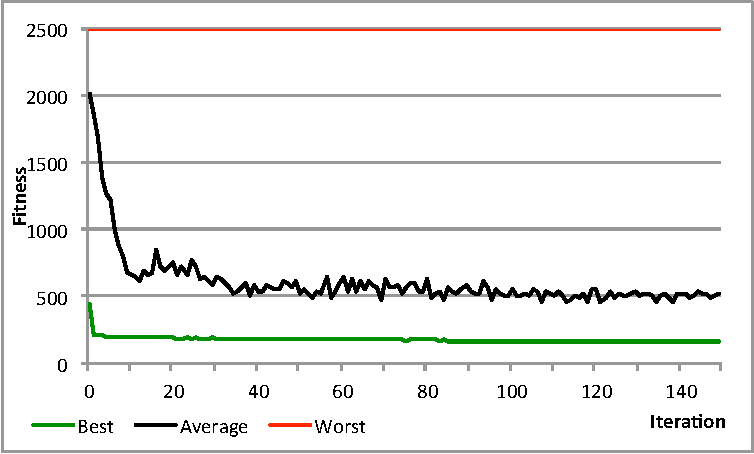
\includegraphics[height=2.5cm]{MC_convergence.pdf} &
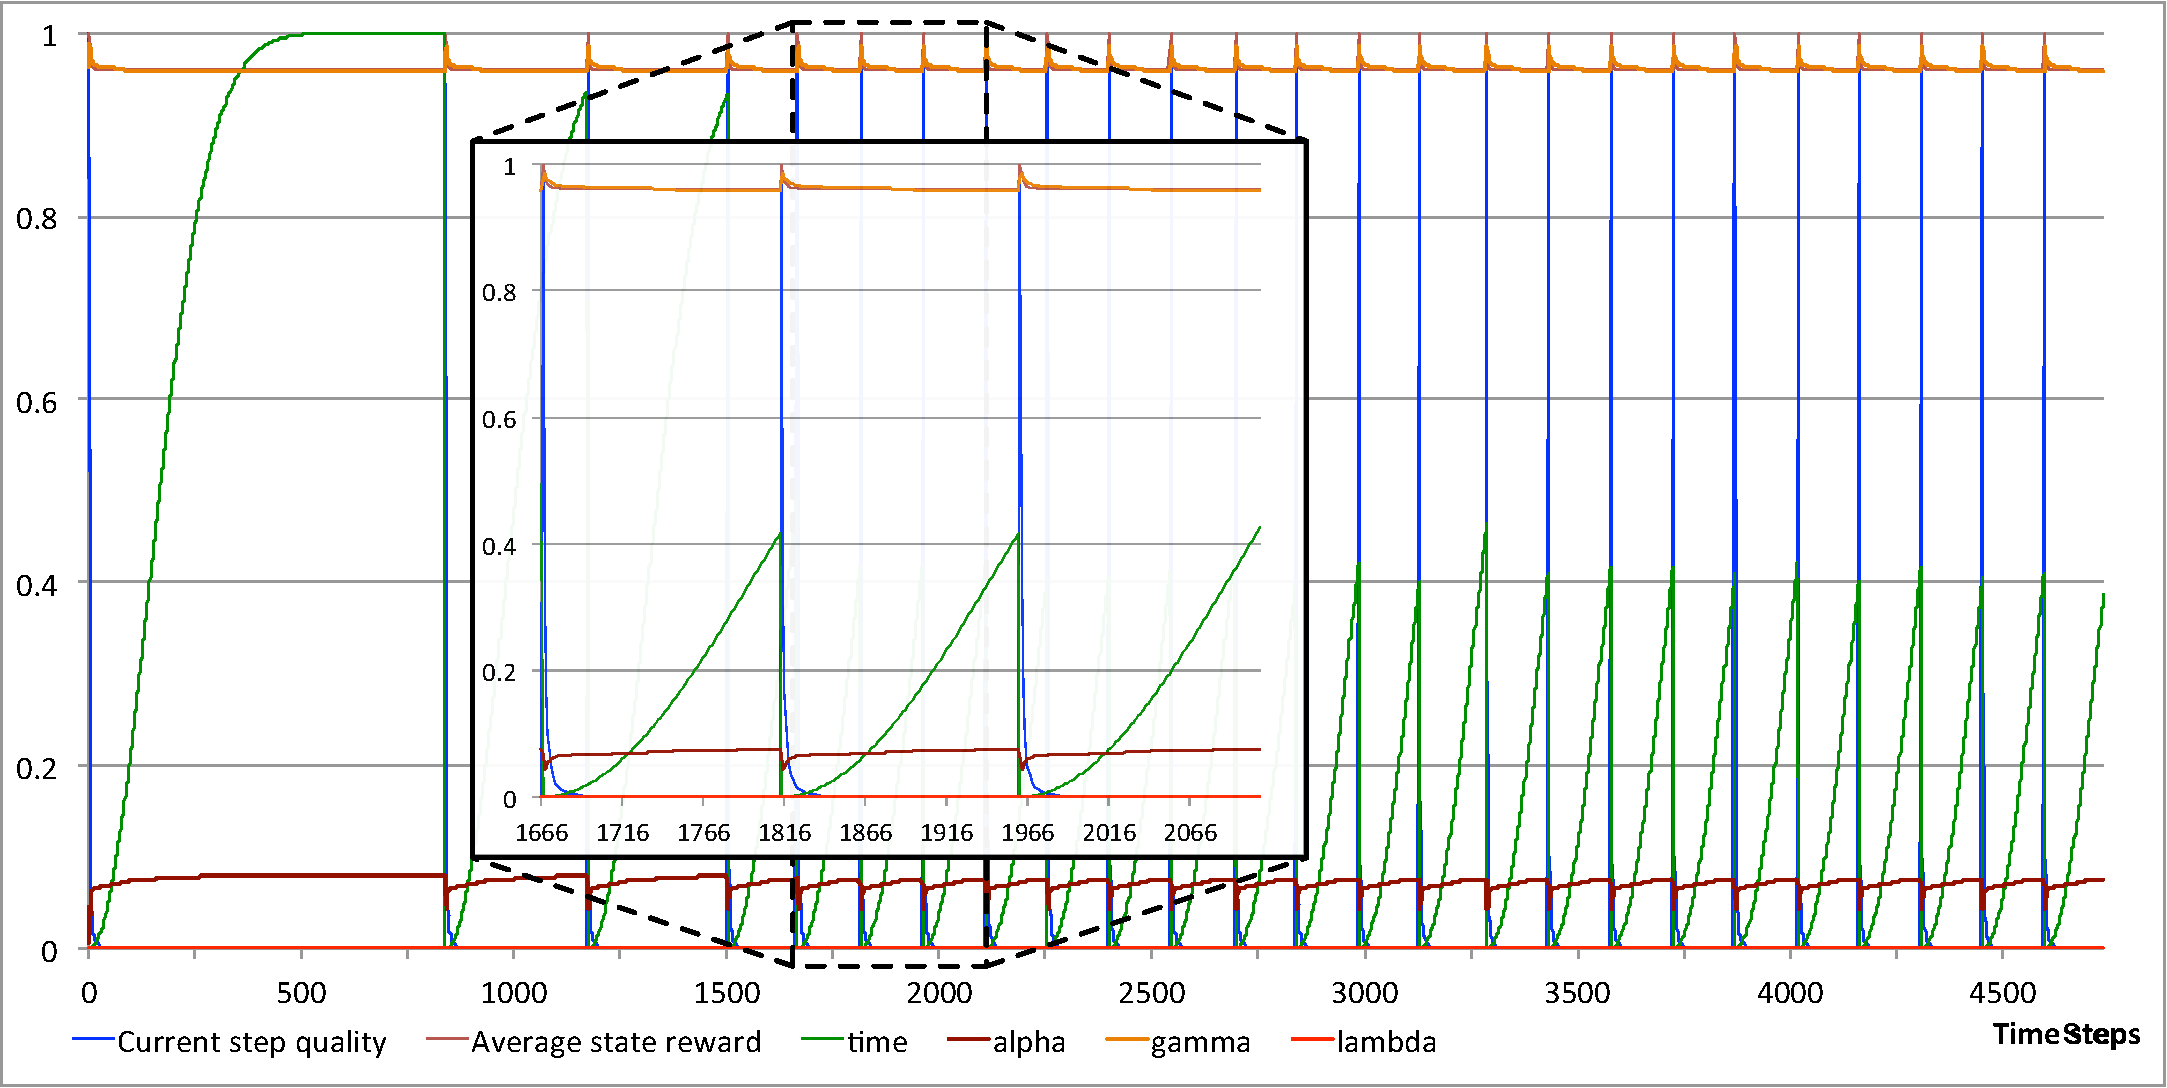
\includegraphics[height=2.5cm]{MC_GRNBehavior.pdf} &
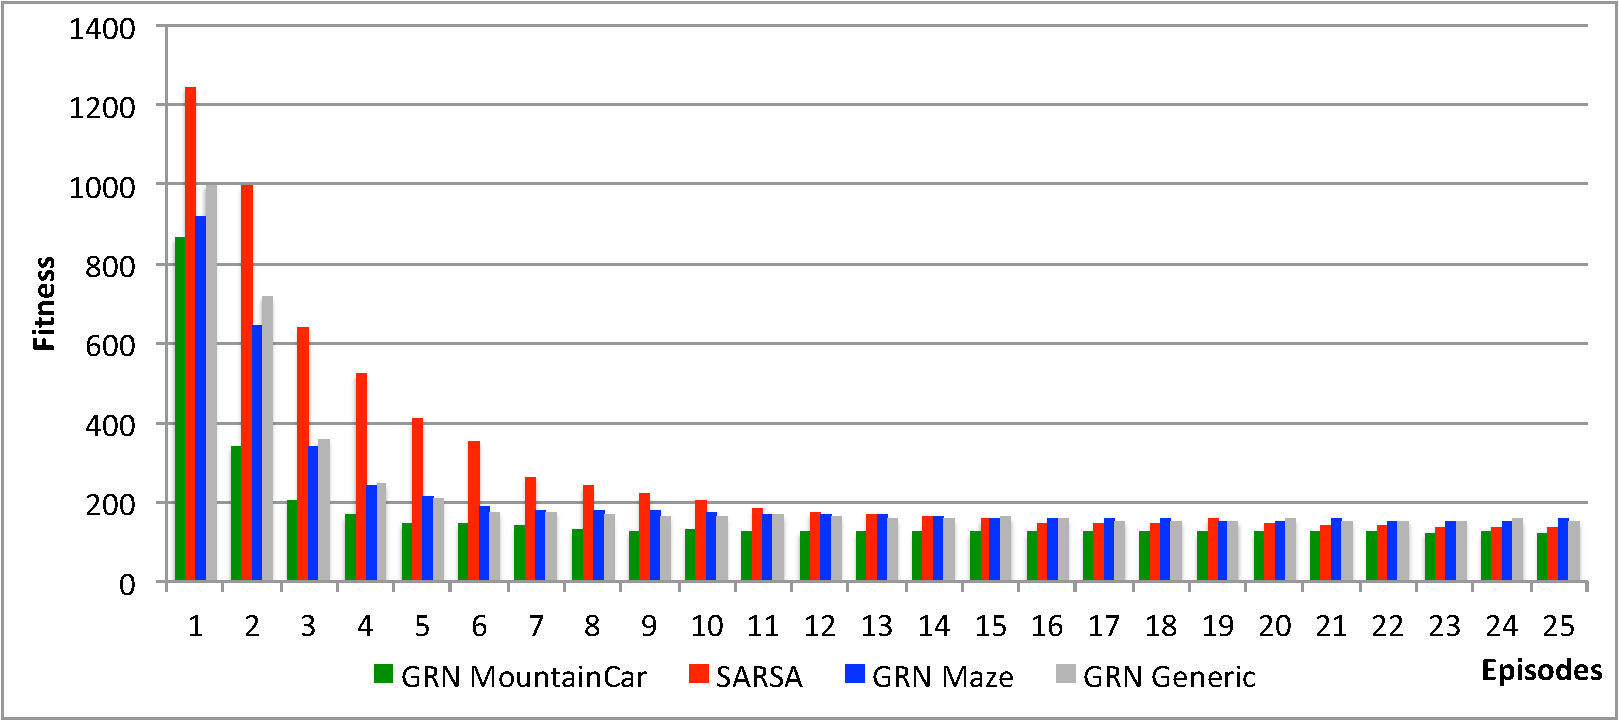
\includegraphics[height=2.5cm]{MC_GRNvsSARSA.pdf}\\
(a) Convergence curve &
(b) Best GRN inputs and outputs &
(c) GRNM vs SARSA
\end{tabular}
\caption{Mountain car: (a) Convergence curve of GRNEAT (lower is better); (b) Regulation of the learning parameters of the best GRN obtained; (c) Comparison of the fitnesses per episode (abscissa) obtained by our neuromodulation with a GRN trained on mountain car (green), with a GRN trained on maze (blue) and with fixed-parameter SARSA algorithm (red). Results are averaged on 100 independent runs. Lower is better.}\label{fig:MC:Results}
\end{figure*}

\subsubsection{Acrobat}

The acrobat problem has a long-standing history in robotics and control, some references to which may be found in \cite{sutton1998introduction}. The agent controls 2 segments with 2 joints, where the first joint represents attachment to the bar, and the second joint represents the waist of the acrobat. The agent can only control the second joint, and the corresponding actions are: apply a fixed amount of positive torque, apply a fixed amount of negative torque, or apply no torque. The agent is initialized in a downward vertical position and must reach an upward vertical position. The agent receives a reward of -1 for each timestep until the episode is complete. This problem is schemetized by figure \ref{fig:ACP:problem}. The fitness is given by the average of rewards received during 30 episodes.

\begin{table}[b]
\center
\begin{tabular}{|c|ccc|}
\cline{2-4}
\multicolumn{1}{c|}{ }	& $\alpha$	& $\gamma$	& $\lambda$	\\\hline
Mountain car			& 0.071429	& 1.0		& 0.928571 	\\%\hline
Maze				& 1.0		& 0.928571	& 0.928571	\\%\hline
Puddle world			&  0.057142	& 0.928571	& 0.5		\\%\hline
Acrobate				& 0.05		& 0.928571	& 0.785714	\\\hline
\end{tabular}
\caption{Fixed learning parameters for the SARSA algorithm obtained by parameter sampling.}\label{tab:SARSAFixedParams}
\end{table}


\subsection{Training GRN on one specific problem}
In this first experiment, we have trained our GRNM model independently on each problem. To evaluate the gain provided by neuromodulation, we first determine the best fixed parameters to use with SARSA on each problem. We use combinatorial parameter sampling on $\alpha$, $\gamma$ and $\lambda$ in $[0, 1]$ with 0.0714 steps (15 evaluations). Each evaluation is averaged on 10 replicates in order to average the randomness of the problems. At the end of the parameter sampling stage, we chose the best fixed learning parameters for a given problem by selecting the tuple with the highest fitness. These parameters are given in Table \ref{tab:SARSAFixedParams}.

\subsubsection{Mountain Car}
Figure \ref{fig:MC:Results}(a) shows the evolutionary convergence curve on the Mountain Car problem. The best GRN is found very quickly (lower green curve) before being slowly optimized to regulate the learning parameters more efficiently. Figure \ref{fig:MC:Results}(b) plots the behavior of the best GRN obtained after 150 iterations. This figure plots the input proteins' concentrations and the three learning parameters calculated by the gene regulatory network. The GRN maintains almost constant parameter values over each episode time, except at the beginning where $\alpha$ and $\gamma$ are increased. This reinforces learned values for the initial part of the agent's trajectory. In this experiment, it should also to be noticed that $\lambda$ is kept at zero all over time, suggesting that on this simple problem sequence learning may not be necessary.

\begin{figure}[b!]
\setlength{\tabcolsep}{0.5mm}
\begin{tabular}{cc}
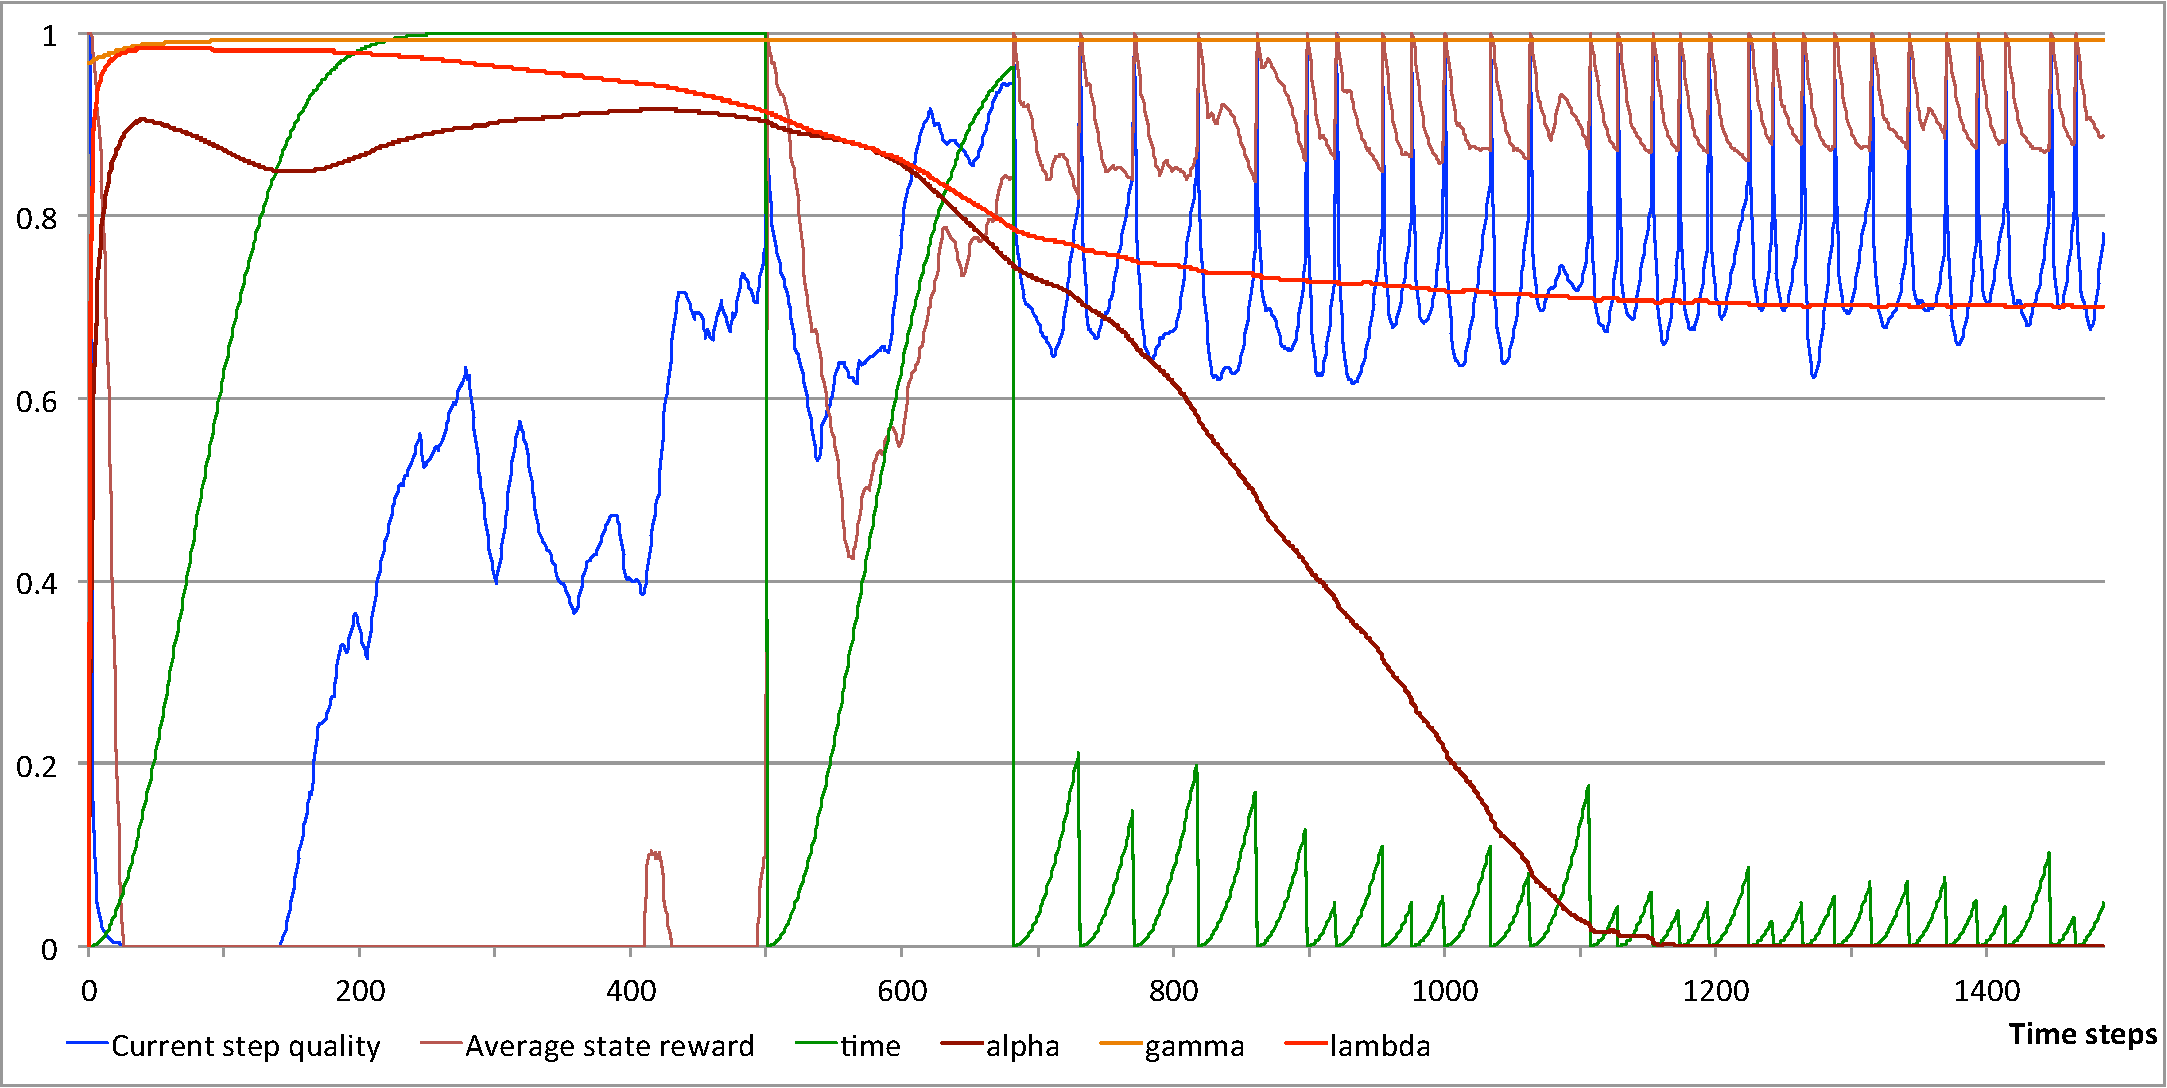
\includegraphics[height=2cm]{MZ_GRNBehavior.pdf}&
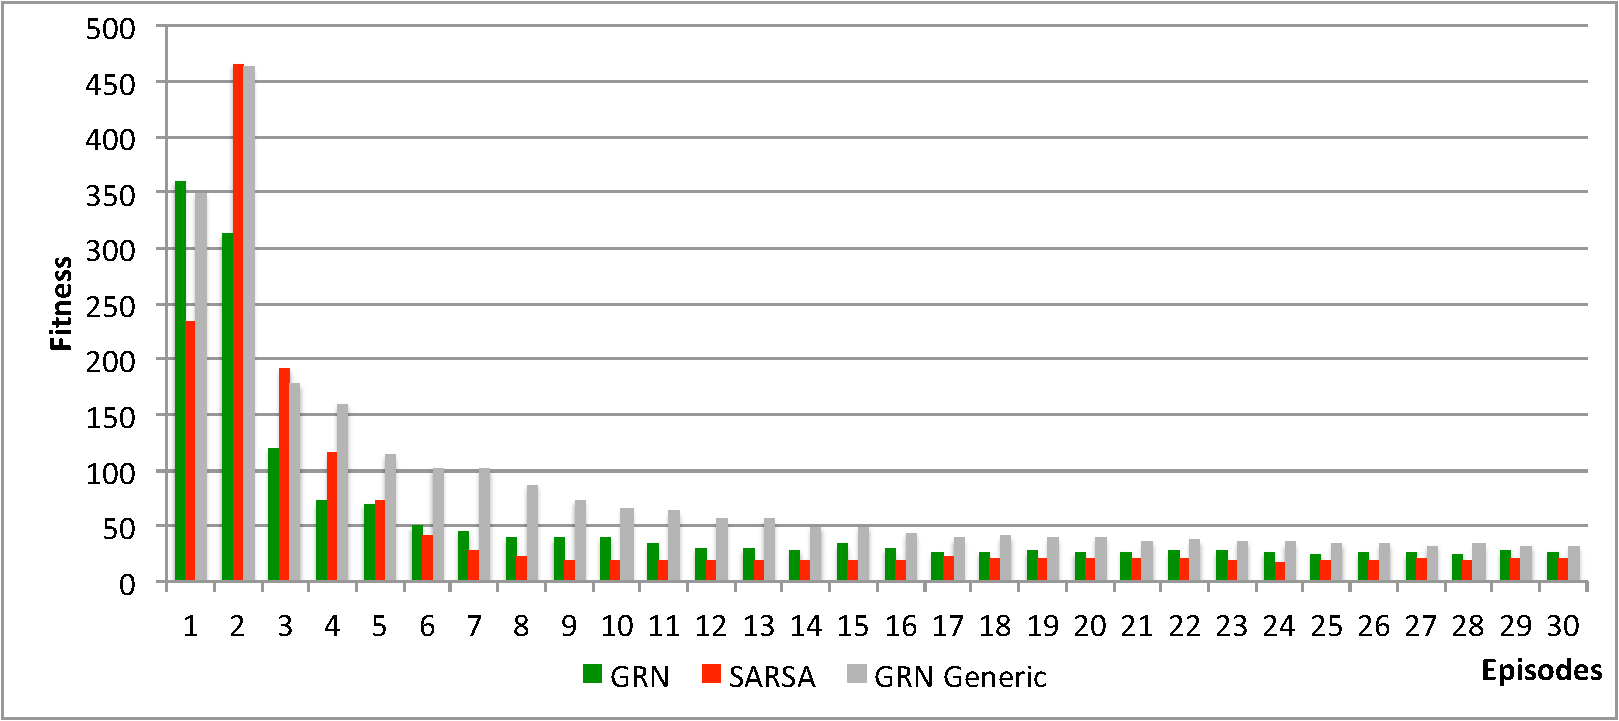
\includegraphics[height=2cm]{MZ_GRNvsSARSA.pdf}\\
(a) Best GRN's behavior &
(b) GRNM vs SARSA
\end{tabular}
\caption{Maze: (a) GRN dynamics of genetically-regulated neuromodulation with the best GRN obtained; (b) Comparison of the fitnesses per episode (abscissa) obtained by GRNM with a GRN trained on Maze (green) and with fixed-parameter SARSA (red). Results are averaged on 100 independent runs. Lower is better.}\label{fig:MZ:Results}
\end{figure}

This GRN is then compared to the SARSA algorithm with fixed learning parameters on 100 independent reruns of mountain car with different random seeds. Figure \ref{fig:MC:Results}(c) shows the results obtained for each episode averaged on the 100 runs. We can observe that GRNM trained on the mountain car (in green) beats the SARSA algorithm with fixed parameters (in red) on every episodes. More specifically, the first episodes (from 1 to 3) show that GRNM learns faster than the SARSA algorithm and later episodes (from 3 to 25) show that neuromodulation leads to agents that solve the problem faster than fixed-parameter SARSA. When comparing detailed results on table \ref{tab:results}, the GRN-based neuromodulation gives better results on the mountain car problem when averaged on 100 independent runs. 

\begin{table*}[t!]
\center
\setlength{\tabcolsep}{.5mm}
\begin{tabular}{|c|cccc|ccc|cccc|cccc|cccc|}
\cline{2-16}
\multicolumn{1}{c}{ }	& \multicolumn{4}{|c}{Mountain Car}	& \multicolumn{3}{|c}{Maze}	 			& \multicolumn{4}{|c}{Puddle World}				& \multicolumn{4}{|c|}{Acrobat} \\
\multicolumn{1}{c|}{ }	
		& GRN	& SARSA	& GRN$_{m}$	& GRN$_{g}$		& GRN$_{m}$	& SARSA	& GRN$_{g}$		& GRN & SARSA & GRN$_{m}$ & GRN$_{g}$		& GRN & SARSA & GRN$_{m}$ & GRN$_{g}$ 			\\\hline
avg		& \textbf{170.5} & 294.2 & \emph{225.3} & 228.3 	& \emph{56.8} & \textbf{53.2} & 83.5	& \textbf{661.9} & \emph{639.0} & 533.7 & 569.5	& \textbf{420.1} & 231.86 & 320.0 & \emph{330.0}		\\
stdev	& \emph{16.7} & \textbf{4.1} & 17.2 & 41.6	  	& \emph{6.1}	& \textbf{4.3}	& 8.4 		& \textbf{105.2} & 234.7 & 177.6 & \emph{175.2}	& \textbf{14.7} & 127.9 & \emph{37.2} & 57.9			\\
best		& \textbf{152.3} & 286.0 & 191.0 & \emph{183.9} 	& \emph{44.0} & \textbf{43.7} & 68.1	& 728.7& \textbf{907.1} & 728.7 & \emph{757.1}	& \emph{453.2} & \textbf{555.0} & 376.7& 404.2		\\
worst	&\textbf{227.4} & 308.1 & \emph{269.6} & 573.2	& \emph{73.2} & \textbf{73.1} & 127.2	& \textbf{281.1}	& -49.5 & 164.6 &	\emph{183.8}	& \textbf{382.2} & 93.5 & \emph{156.8}& 149.3		\\\hline
\end{tabular}
\caption{Detailed results of the 100 runs from the four problems with the best GRN trained on the specific problem, the SARSA algorithm with fixed parameters, the GRN trained on Maze (noted GRN$_{m}$ in the table), and a generic GRN trained both on the Maze and Mountain Car problems (noted GRN$_{g}$). Notice that, for the first two problems (Mountain Car and Maze), lower is better and for the two others (Puddle World and Acrobat), higher is better. Bold values are best per problem, per row. Italics indicate second best.}\label{tab:results}
\end{table*}

\begin{figure*}[b!]
\center
\begin{minipage}[t!]{0.49\linewidth}
\center
\setlength{\tabcolsep}{0.5mm}
\begin{tabular}{cc}
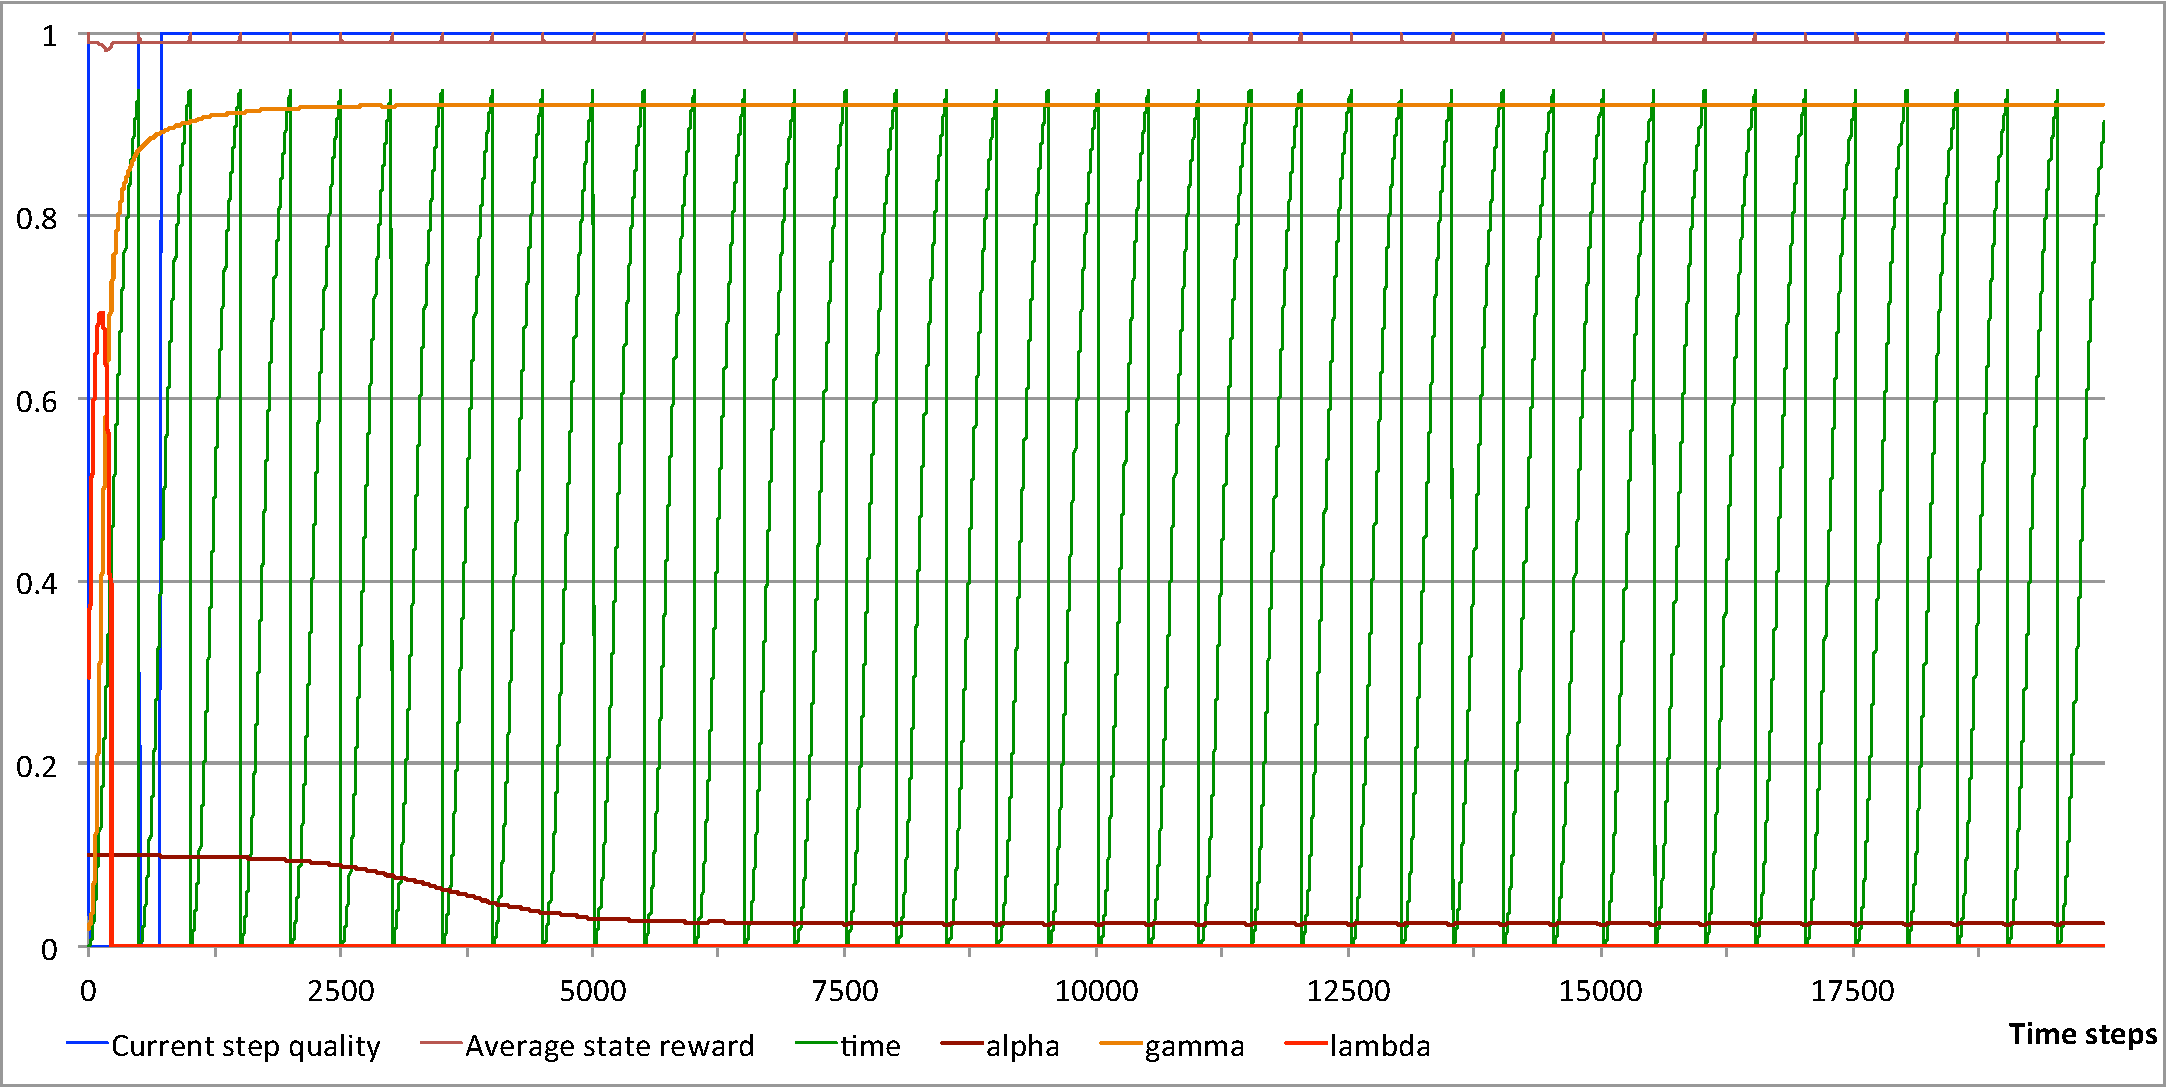
\includegraphics[height=2cm]{PW_GRNBehavior.pdf} &
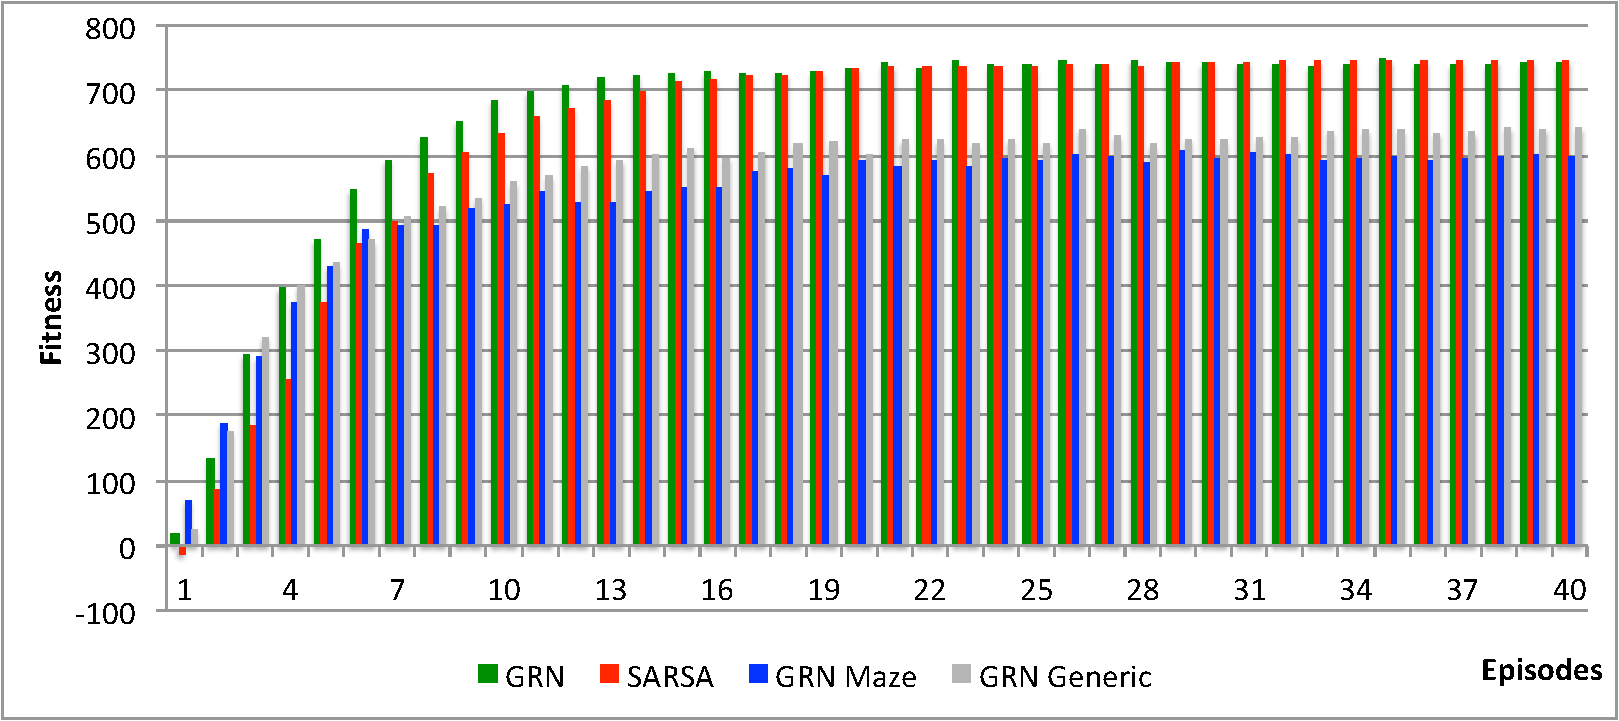
\includegraphics[height=2cm]{PW_GRNvsSARSA.pdf} \\
(a) Best GRN's behavior &
(b) GRNM vs SARSA
\end{tabular}
\caption{Puddle World: (b) Comparison of the fitnesses per episode (abscissa) obtained by genetically-regulated neuromodulation with a GRN trained on this problem (green), a GRN trained on Maze (blue), a GRN trained on Maze and Mountain Car (gray) and with the fixed-parameter SARSA algorithm (red). Results are averaged on 100 independent runs. Higher is better.}\label{fig:PW:Results}
\end{minipage}
\hspace{1.5mm}
%%%%%%
\begin{minipage}[t!]{0.49\linewidth}
\center
\setlength{\tabcolsep}{0.5mm}
\begin{tabular}{cc}
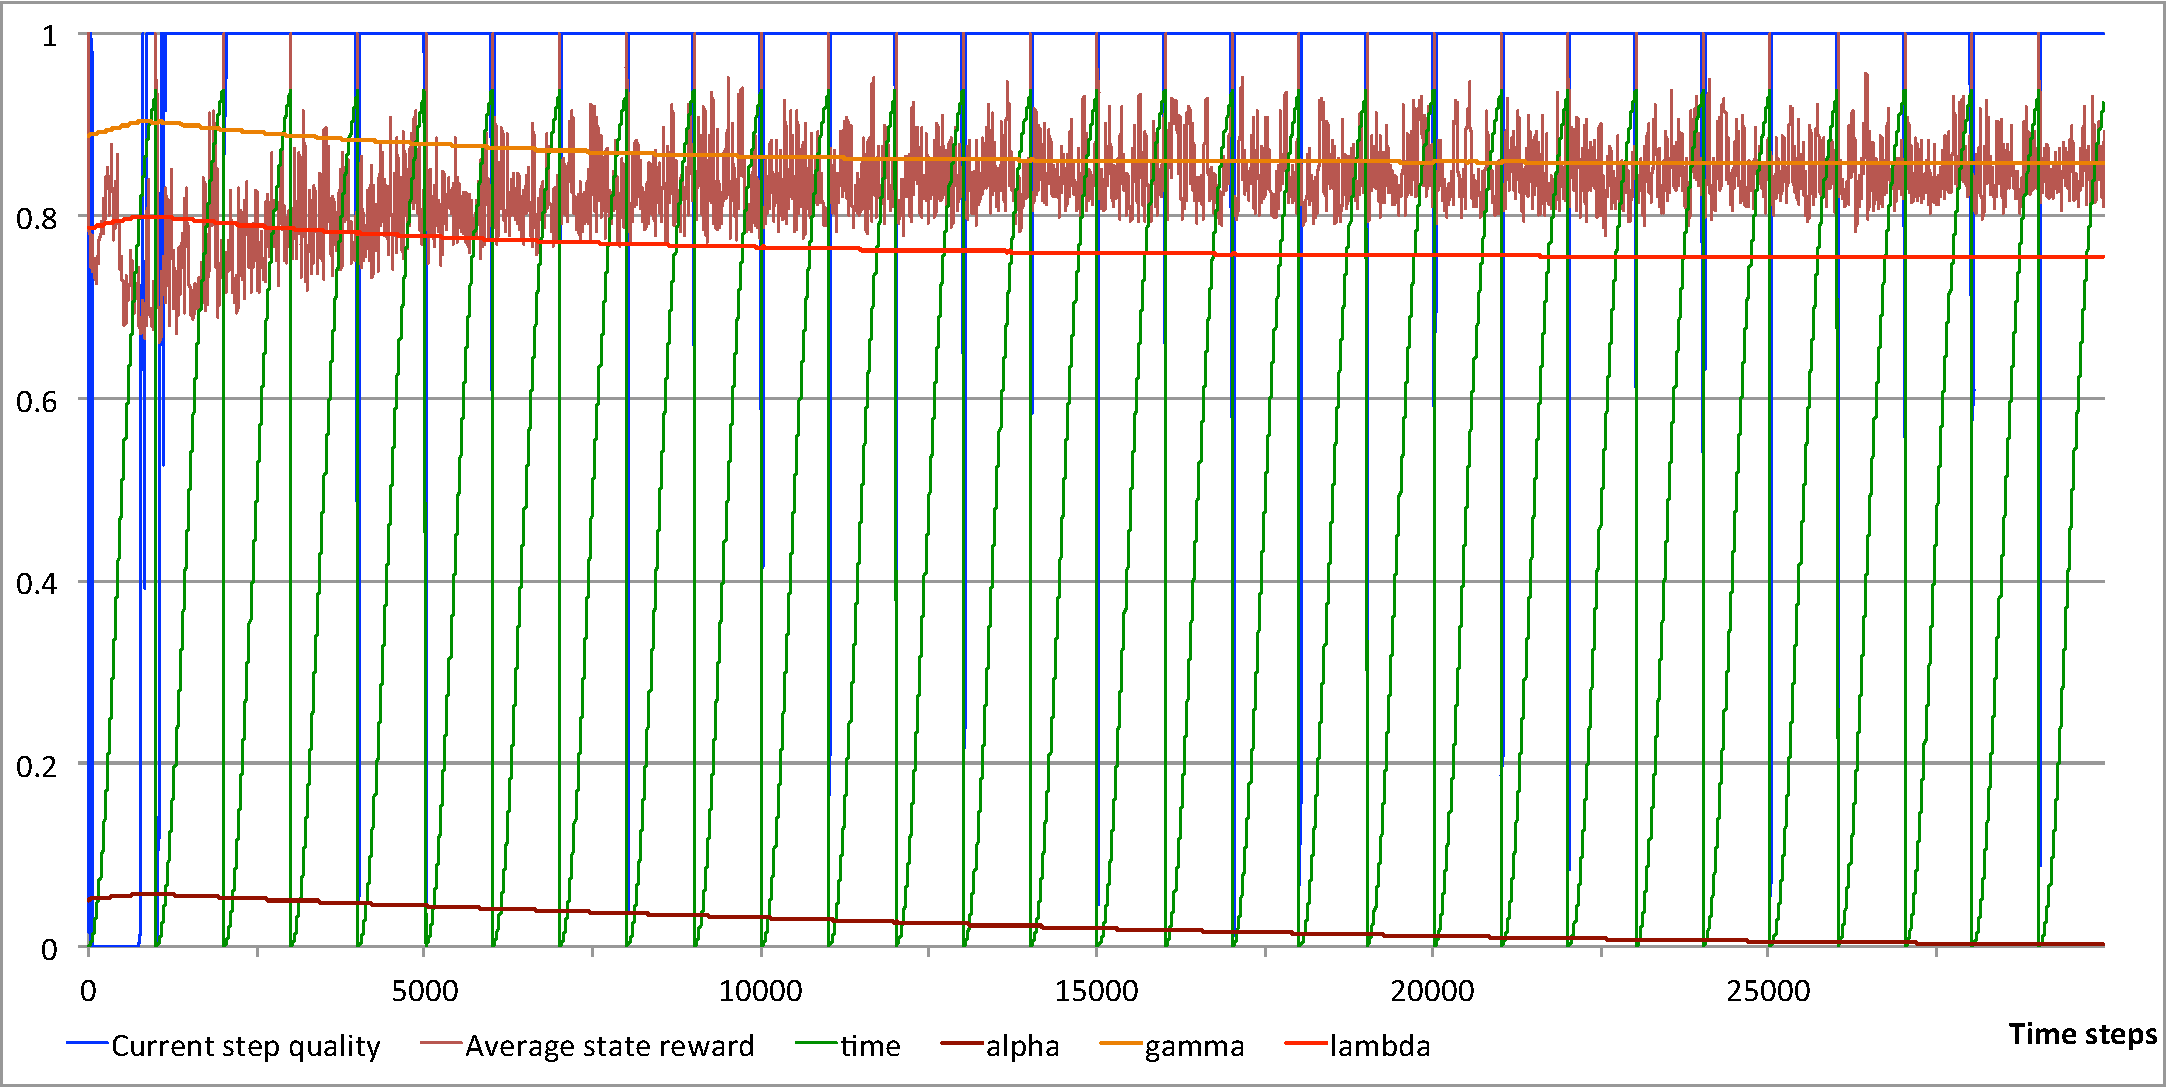
\includegraphics[height=2cm]{ACP_GRNBehavior.pdf} &
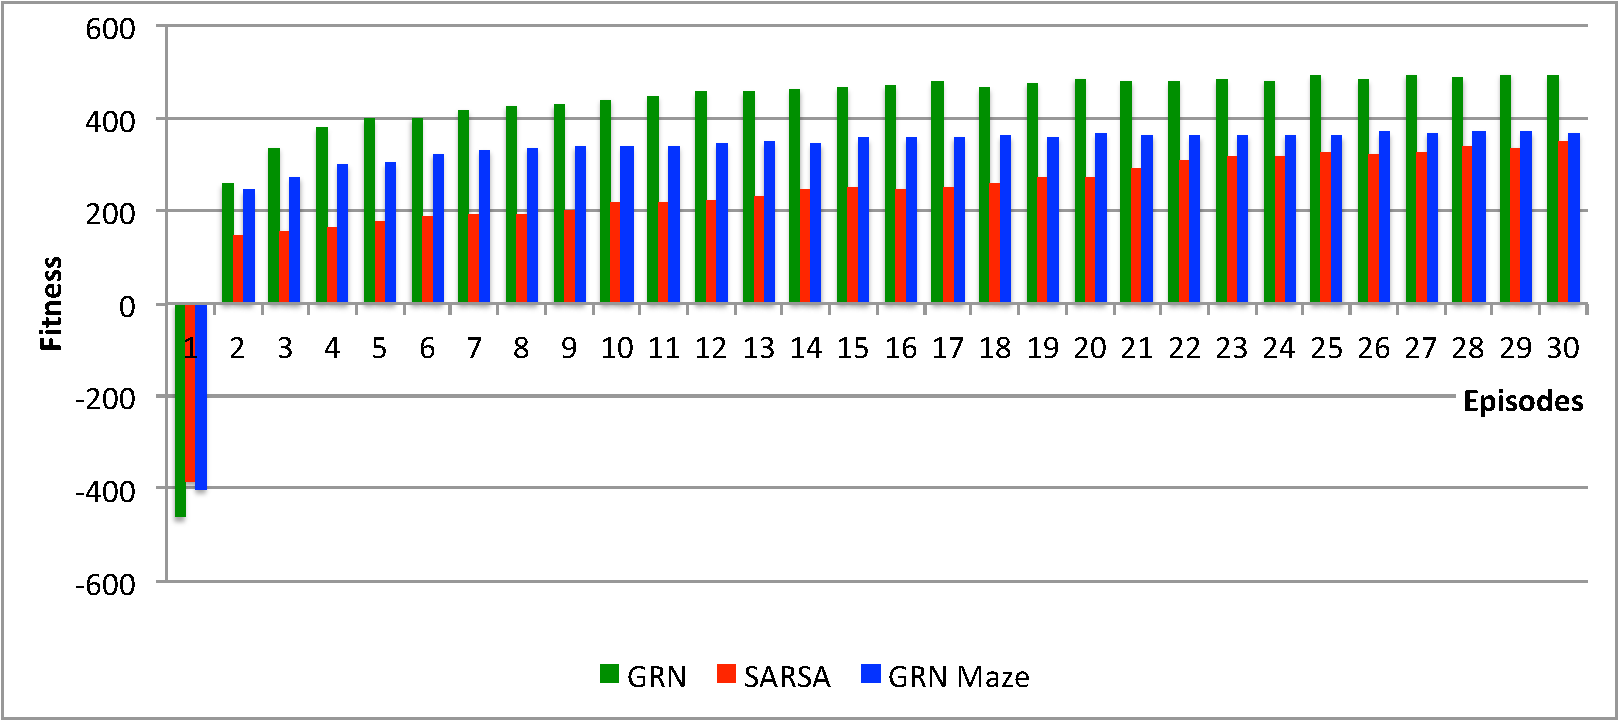
\includegraphics[height=2cm]{ACP_GRNvsSARSA.pdf} \\
(a) Best GRN's behavior &
(b) GRNM vs SARSA
\end{tabular}
\caption{Acrobat: (a) Regulation of the learning parameters of the best GRN obtained; (b) Comparison of the fitnesses per episode (abscissa) obtained by genetically-regulated neuromodulation with a GRN trained on this problem (green) and a GRN trained on Maze (blue) and with the fixed-parameter SARSA algorithm (red). Results are averaged on 100 independent runs. Higher is better. }\label{fig:ACP:Results}
\end{minipage}
\end{figure*}

\subsubsection{Maze}
The same procedure has been used to evolve a gene regulatory network to regulate SARSA algorithm's learning parameters on the Maze problem. Figure \ref{fig:MZ:Results}(a) presents the behavior of the best GRN obtained after evolution. The regulatory dynamics differ significantly from those obtained on the Mountain Car problem. This GRN starts with very high values for all learning parameters leading to a strong memorization of initial experiences. Then, upon discovering successful solutions, the learning rate $\alpha$ and the memory depth $\lambda$ decrease to exploit the learned behaviors. $\gamma$ is kept very high all along the simulation.

When compared to the fixed-parameter SARSA algorithm (figure \ref{fig:MZ:Results}(b)), we can observe that GRNM is learning faster than the SARSA algorithm (episodes 2 to 5). However, the advantage turns to the fixed-parameter SARSA algorithm in the remaining episodes: the latter is doing slightly better than GRNM from episode 6 to the end. When referring to the detailed results given by table \ref{tab:results}, GRNM and fixed-parameter SARSA give comparable results. 

\subsubsection{Puddle World}
Figure \ref{fig:PW:Results}(a) presents the behavior of the best GRN obtained when neuromodulation is optimized on the puddle world problem. Once again, the GRN chooses to use higher learning parameters $\alpha$ and $\lambda$ at the beginning of the simulation to learn from initial experiences  faster. After this initial phase, the GRN increases the discounting factor and reduces the amount of memorization in order to better exploit learned experiences. This gives good results in comparison to fixed-parameter SARSA: as depicted in figure \ref{fig:PW:Results}(b), GRNM learns the value of states and actions faster and converges to an equivalent solution to fixed-parameter SARSA. When comparing the results in detail (table \ref{tab:results}), neuromodulation obtains equivalent results when averaged on 100 independent runs but the standard deviation and worst result are better: the GRNM is capable of modulating the learning parameters when harder scenarios are encountered. 

\subsubsection{Acrobat}

Figure \ref{fig:ACP:Results}(a) shows the regulation obtained with the best GRN evolved on the acrobat problem. The GRN finds learning parameters very close to the one obtained with parameter sampling for the fixed-parameter SARSA algorithm. However, in addition to finding these parameters, the GRN reduces these values all along the episodes, in particular $\alpha$ which decreases down to zero. As in the puddle world problem, the aim is to exploit more the results when an appropriate behavior is found by the SARSA algorithm. When compared to the fixed-parameter SARSA algorithm on this problem (figure \ref{fig:ACP:Results}(b)), GRN-based neuromodulation both learns faster and finishes with a better behavior than the fixed-parameter SARSA algorithm. This is confirmed by table \ref{tab:results} in which the reward averaged on 100 independent runs is largely over with neuromodulation than with the fixed-parameter SARSA algorithm. 


\begin{figure*}[t!]
\center
\begin{tabular}{ccc}
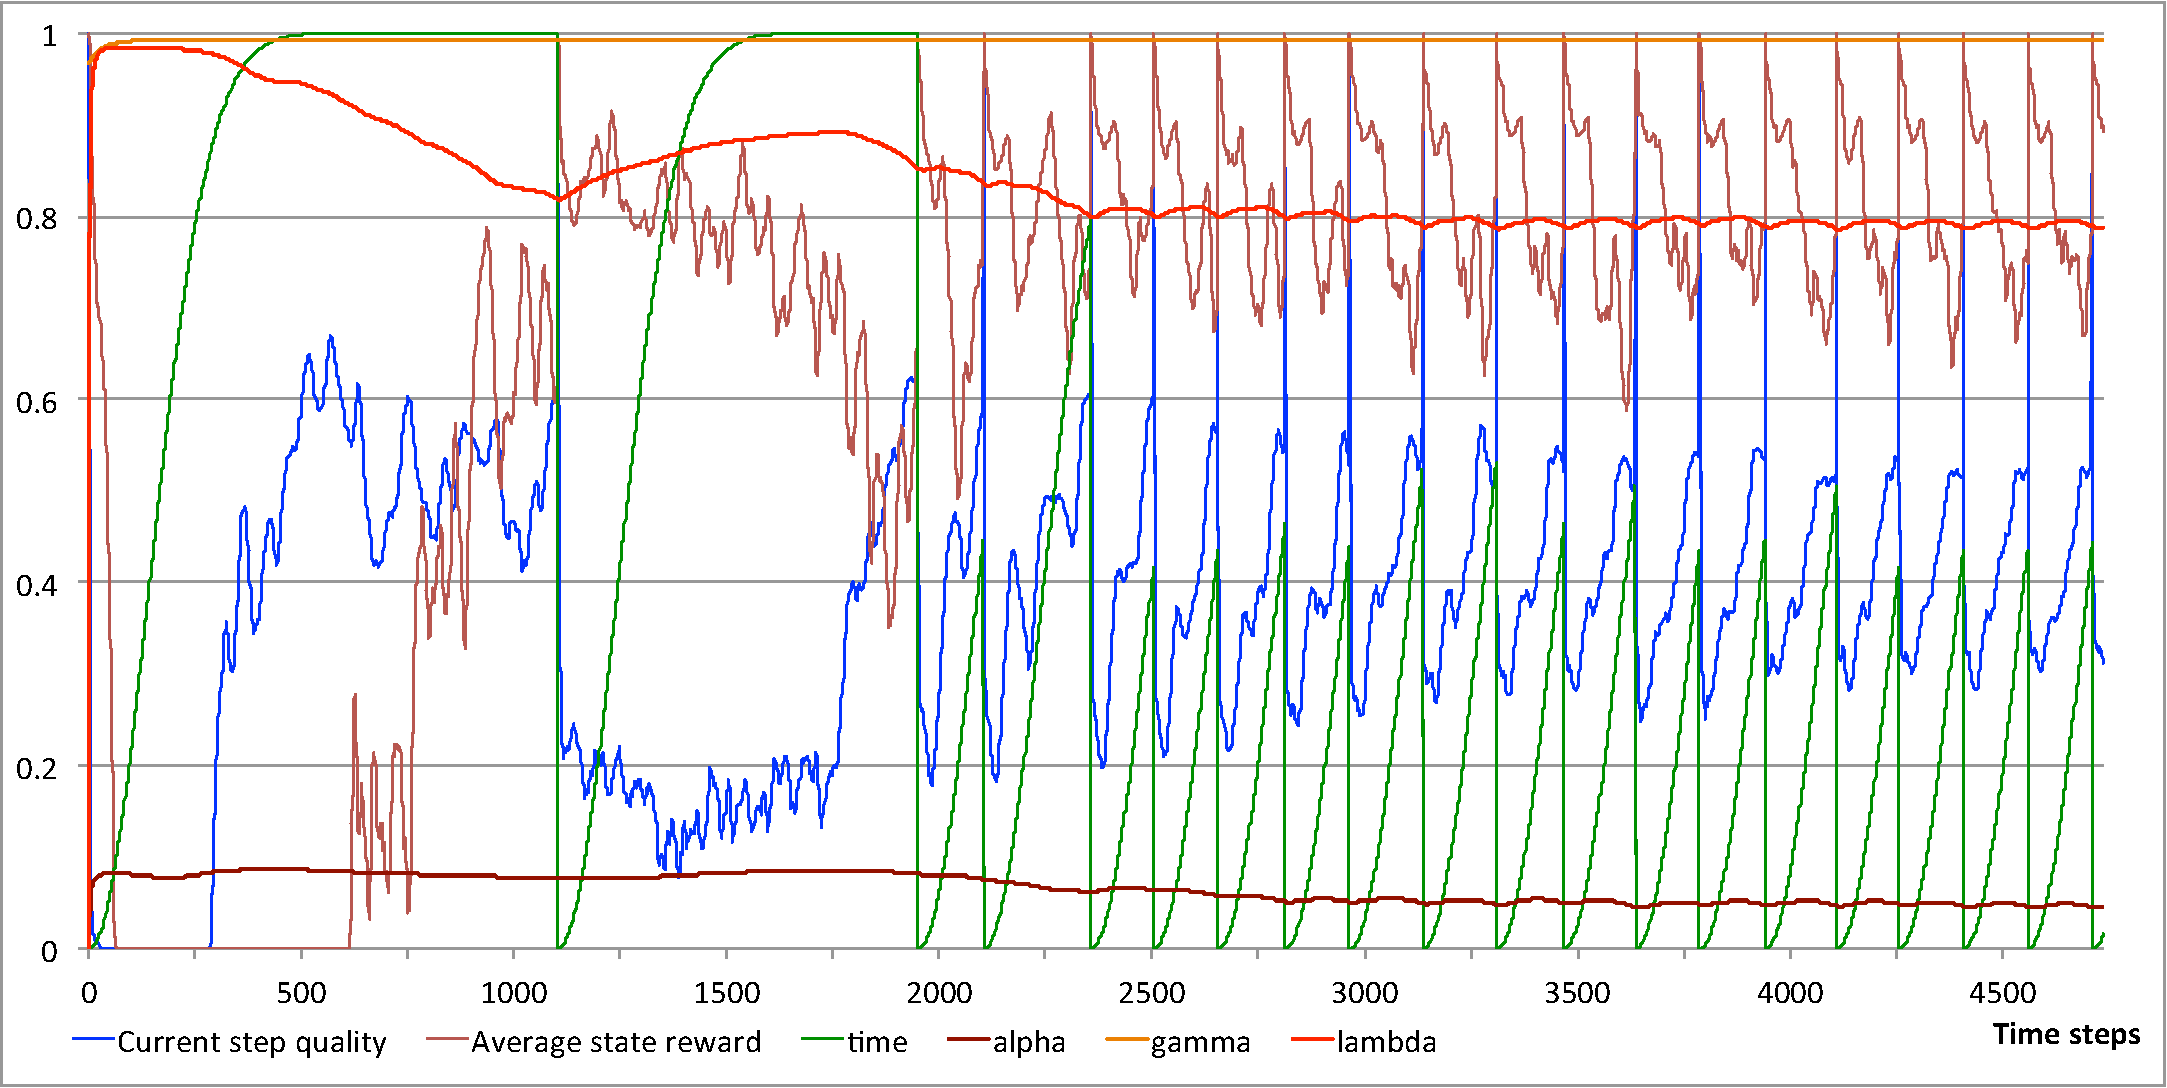
\includegraphics[width=0.32\linewidth]{MC_GRNMazeBehavior.pdf} &
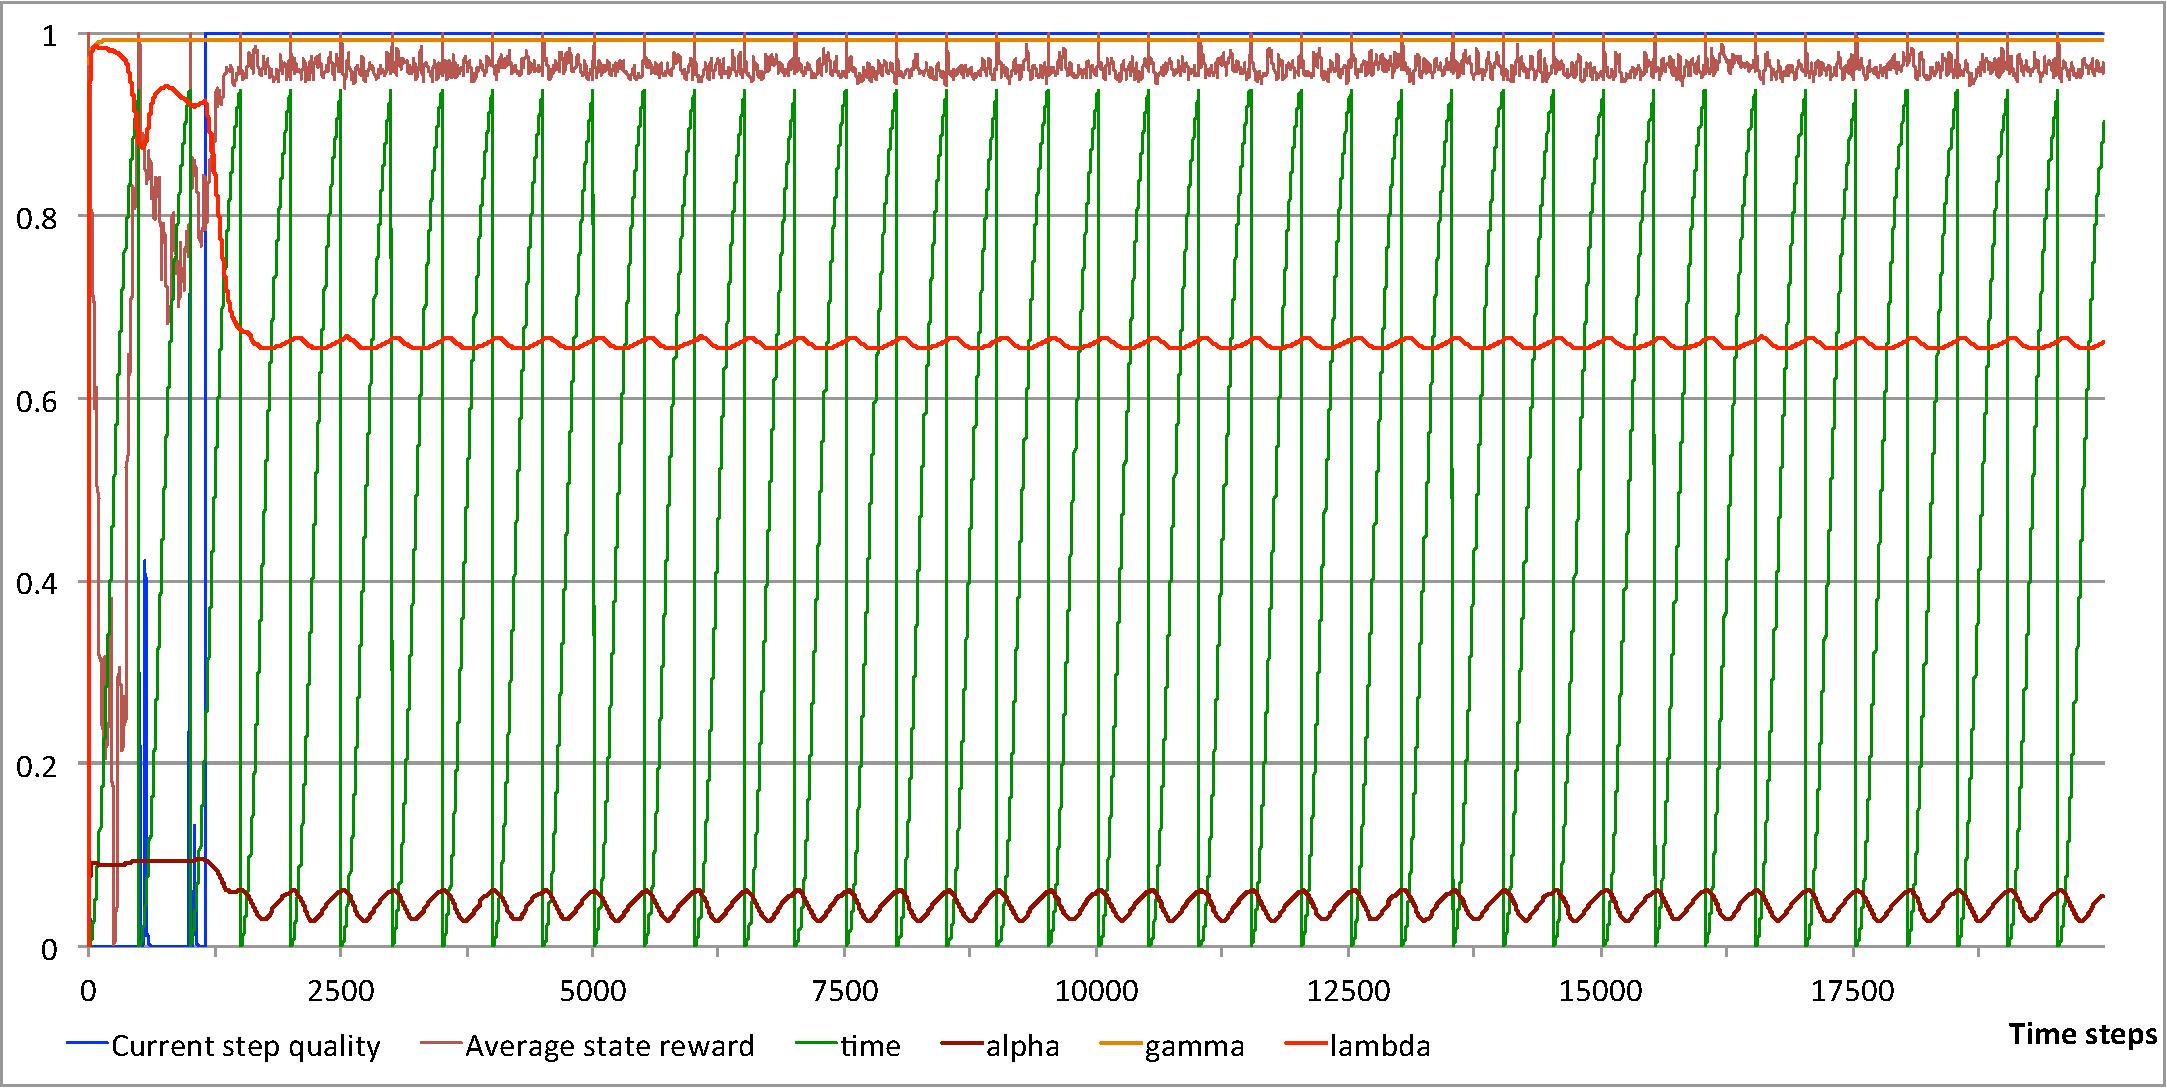
\includegraphics[width=0.32\linewidth]{PW_GRNMazeBehavior.pdf} &
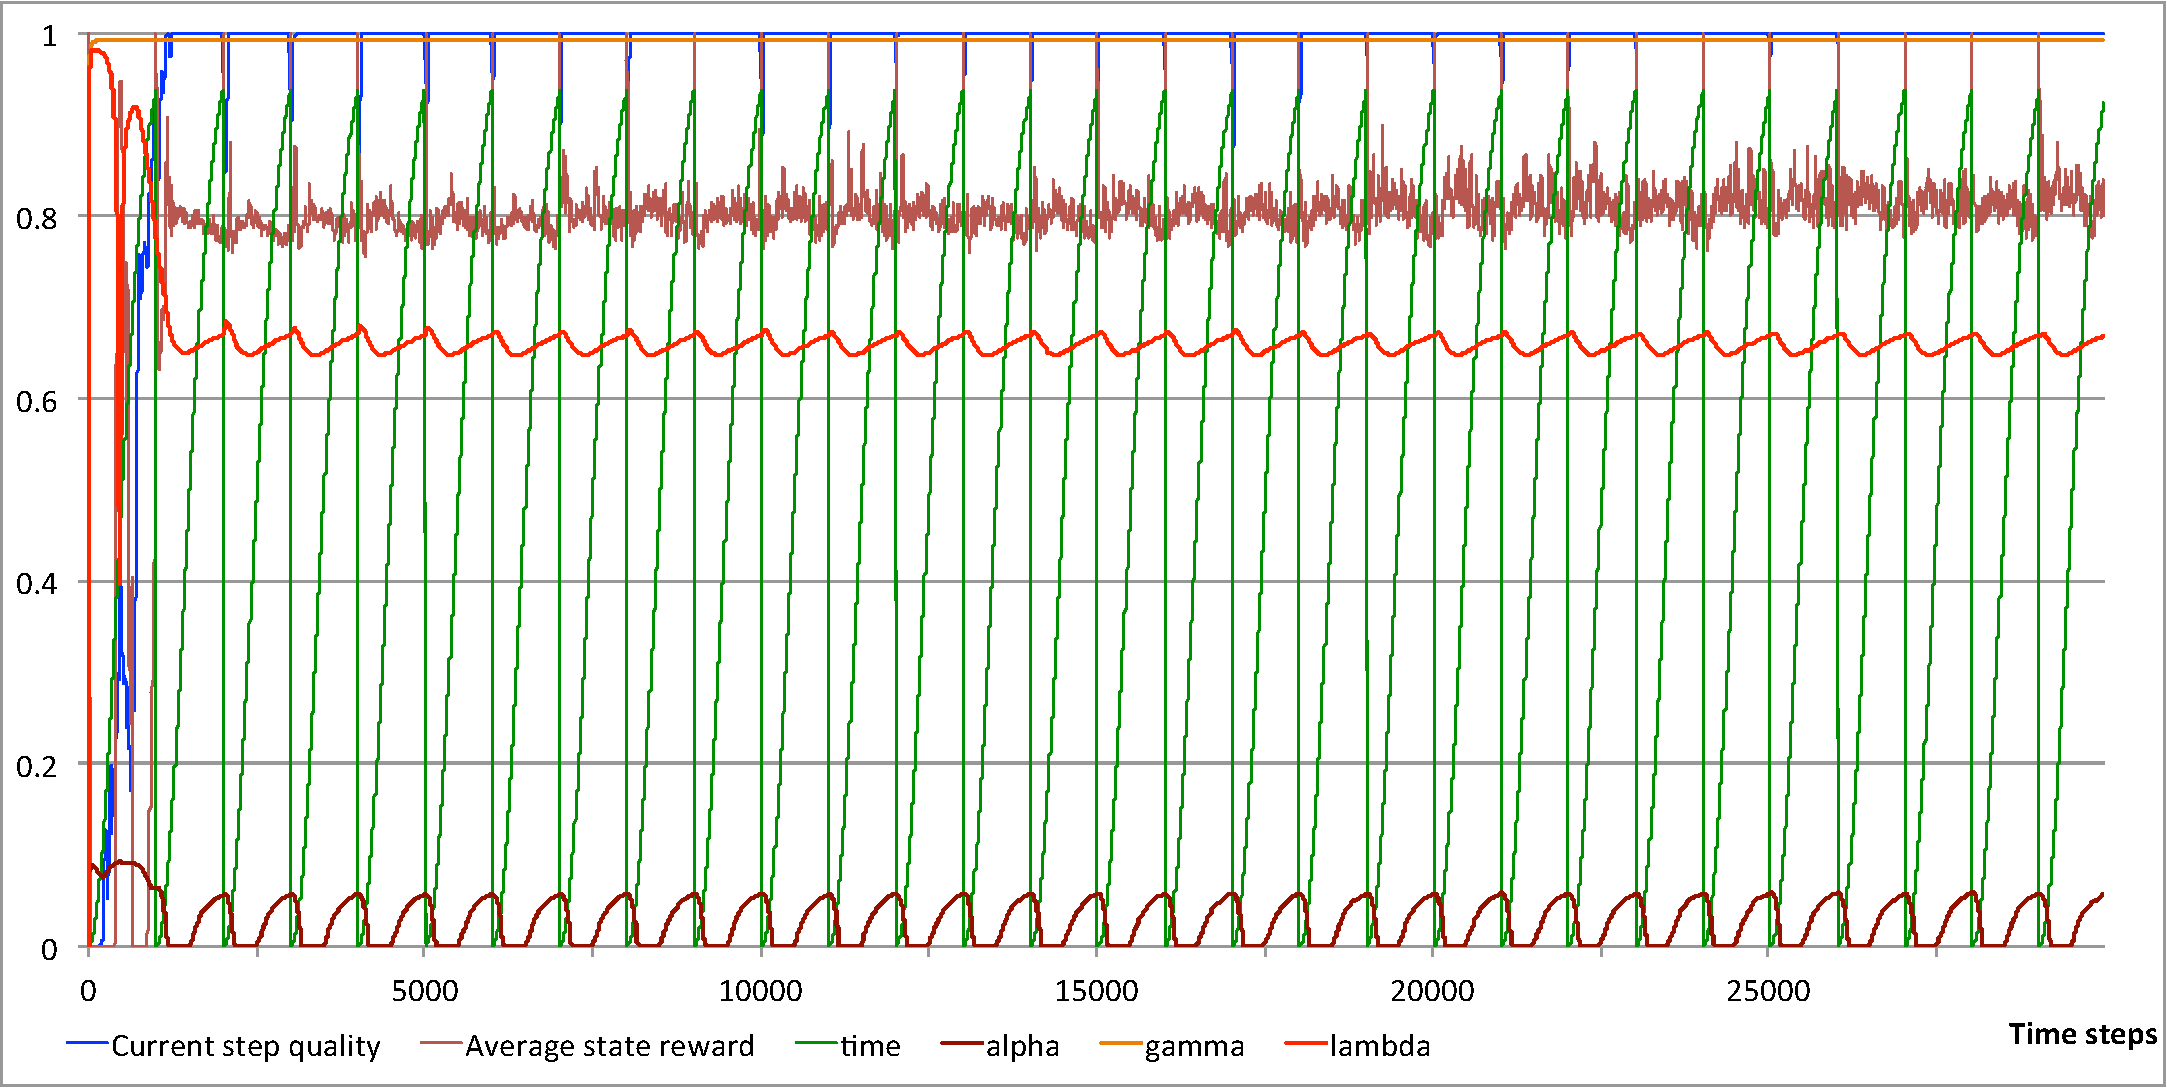
\includegraphics[width=0.32\linewidth]{ACP_GRNMazeBehavior.pdf} \\
(a) Mountain Car & (b) Puddle World & (c) Acrobat
\end{tabular}
\caption{Behavior of the GRN trained on the Maze problem when used to regulate learning parameters on Mountain Car, Puddle World and Acrobat.}\label{fig:all:GRNMazeBehavior}
\end{figure*}

\begin{figure*}[b!]
\center
\setlength{\tabcolsep}{0.5mm}
\begin{tabular}{cccc}
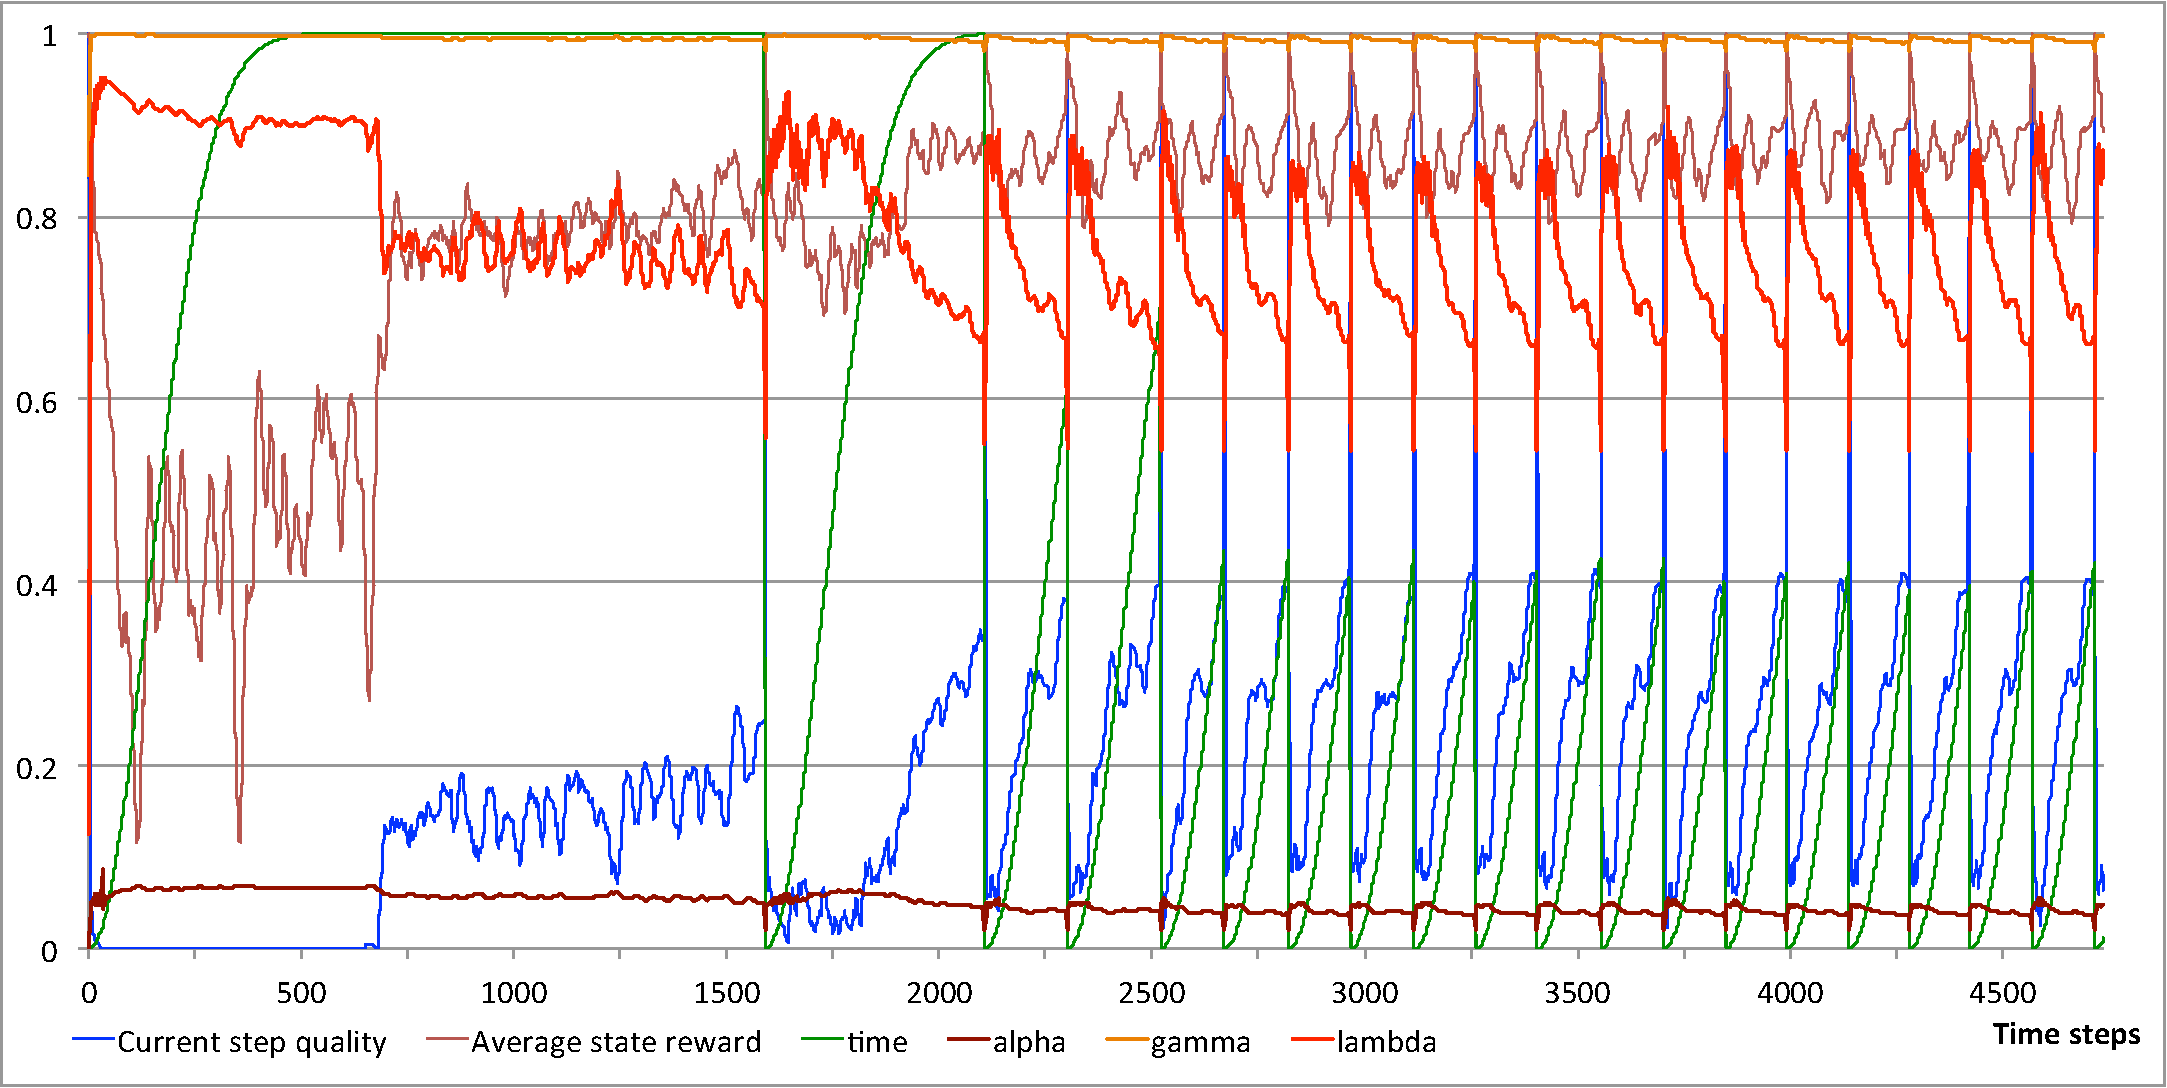
\includegraphics[width=0.245\linewidth]{MC_GRNGenericBehavior.pdf} &
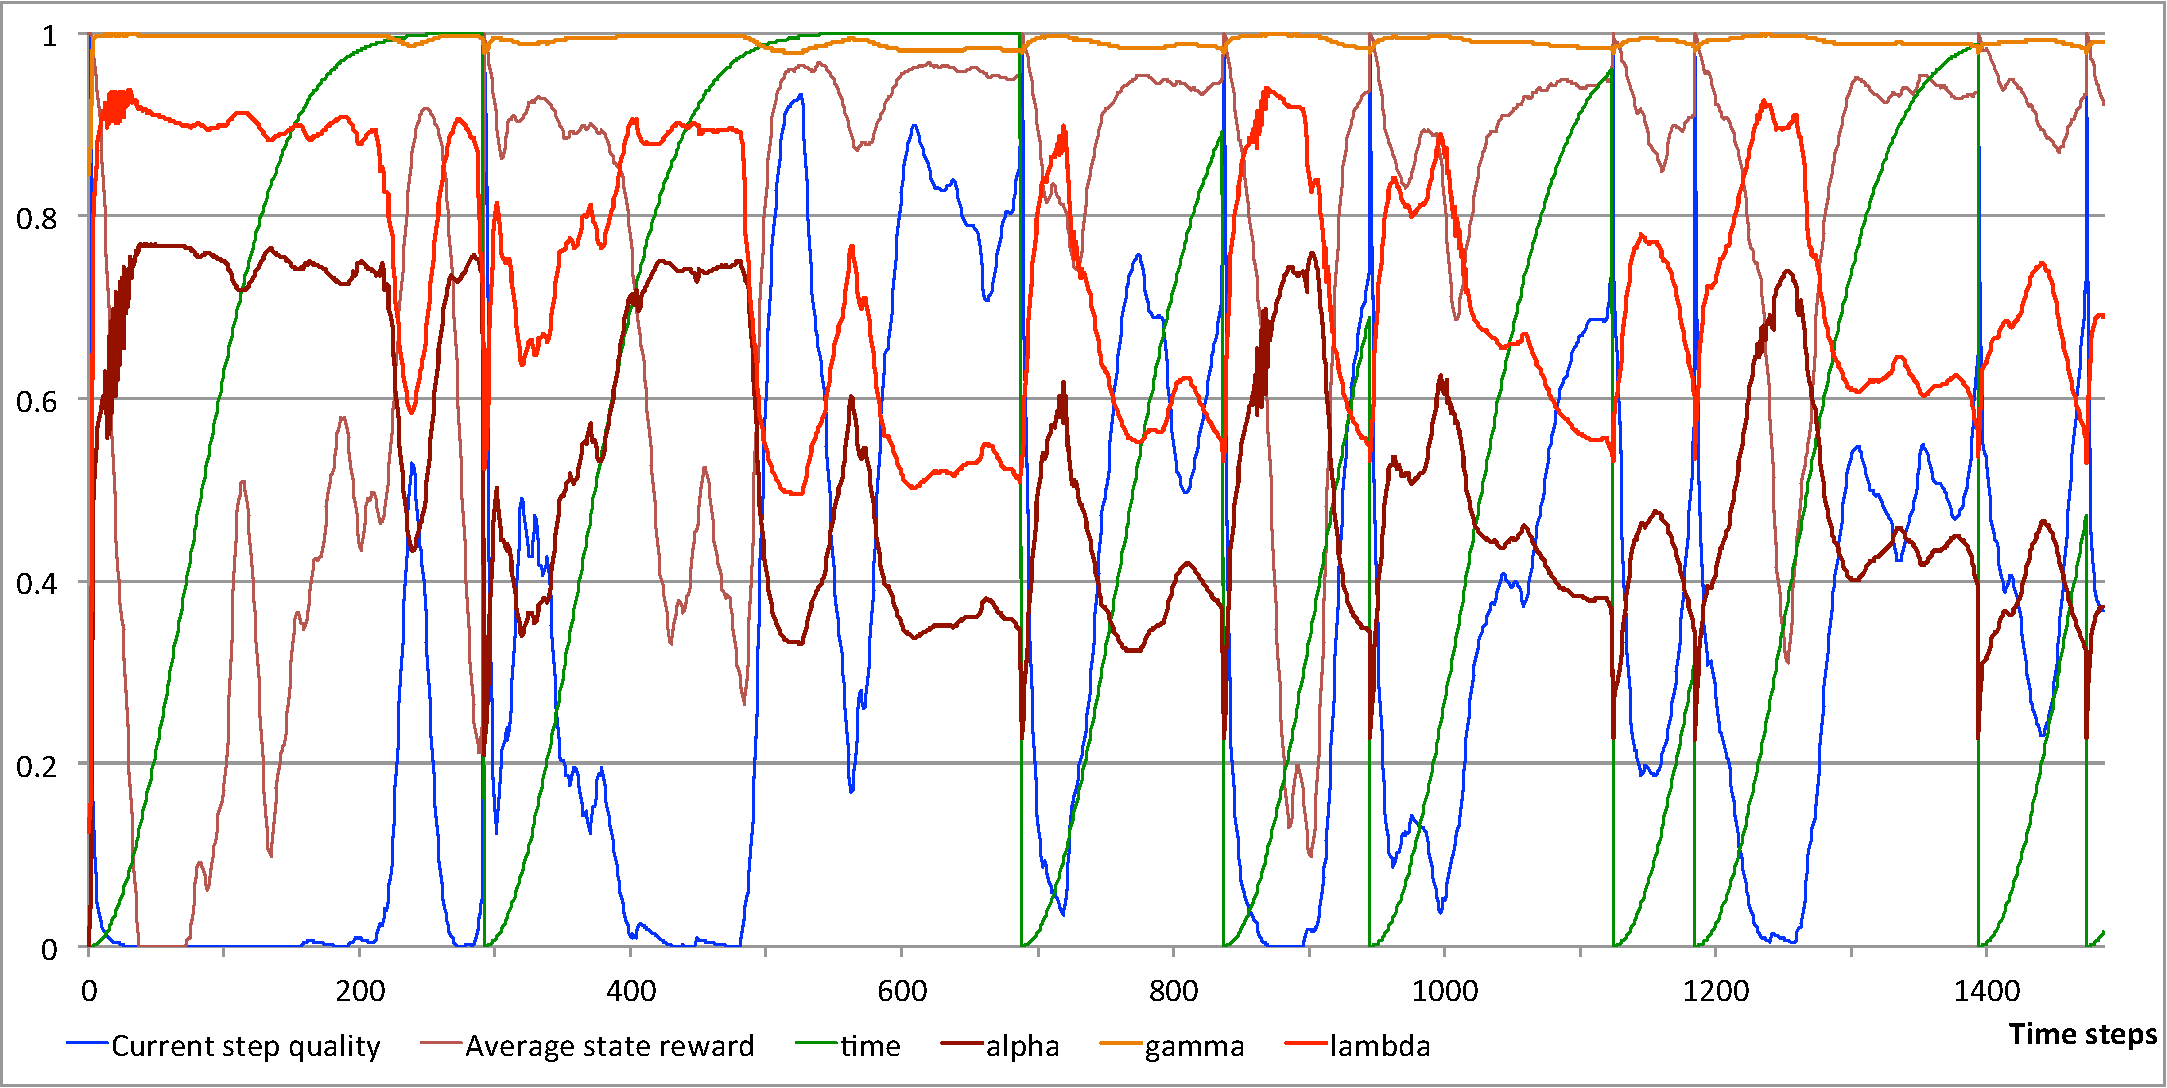
\includegraphics[width=0.245\linewidth]{MZ_GRNGenericBehavior.pdf} &
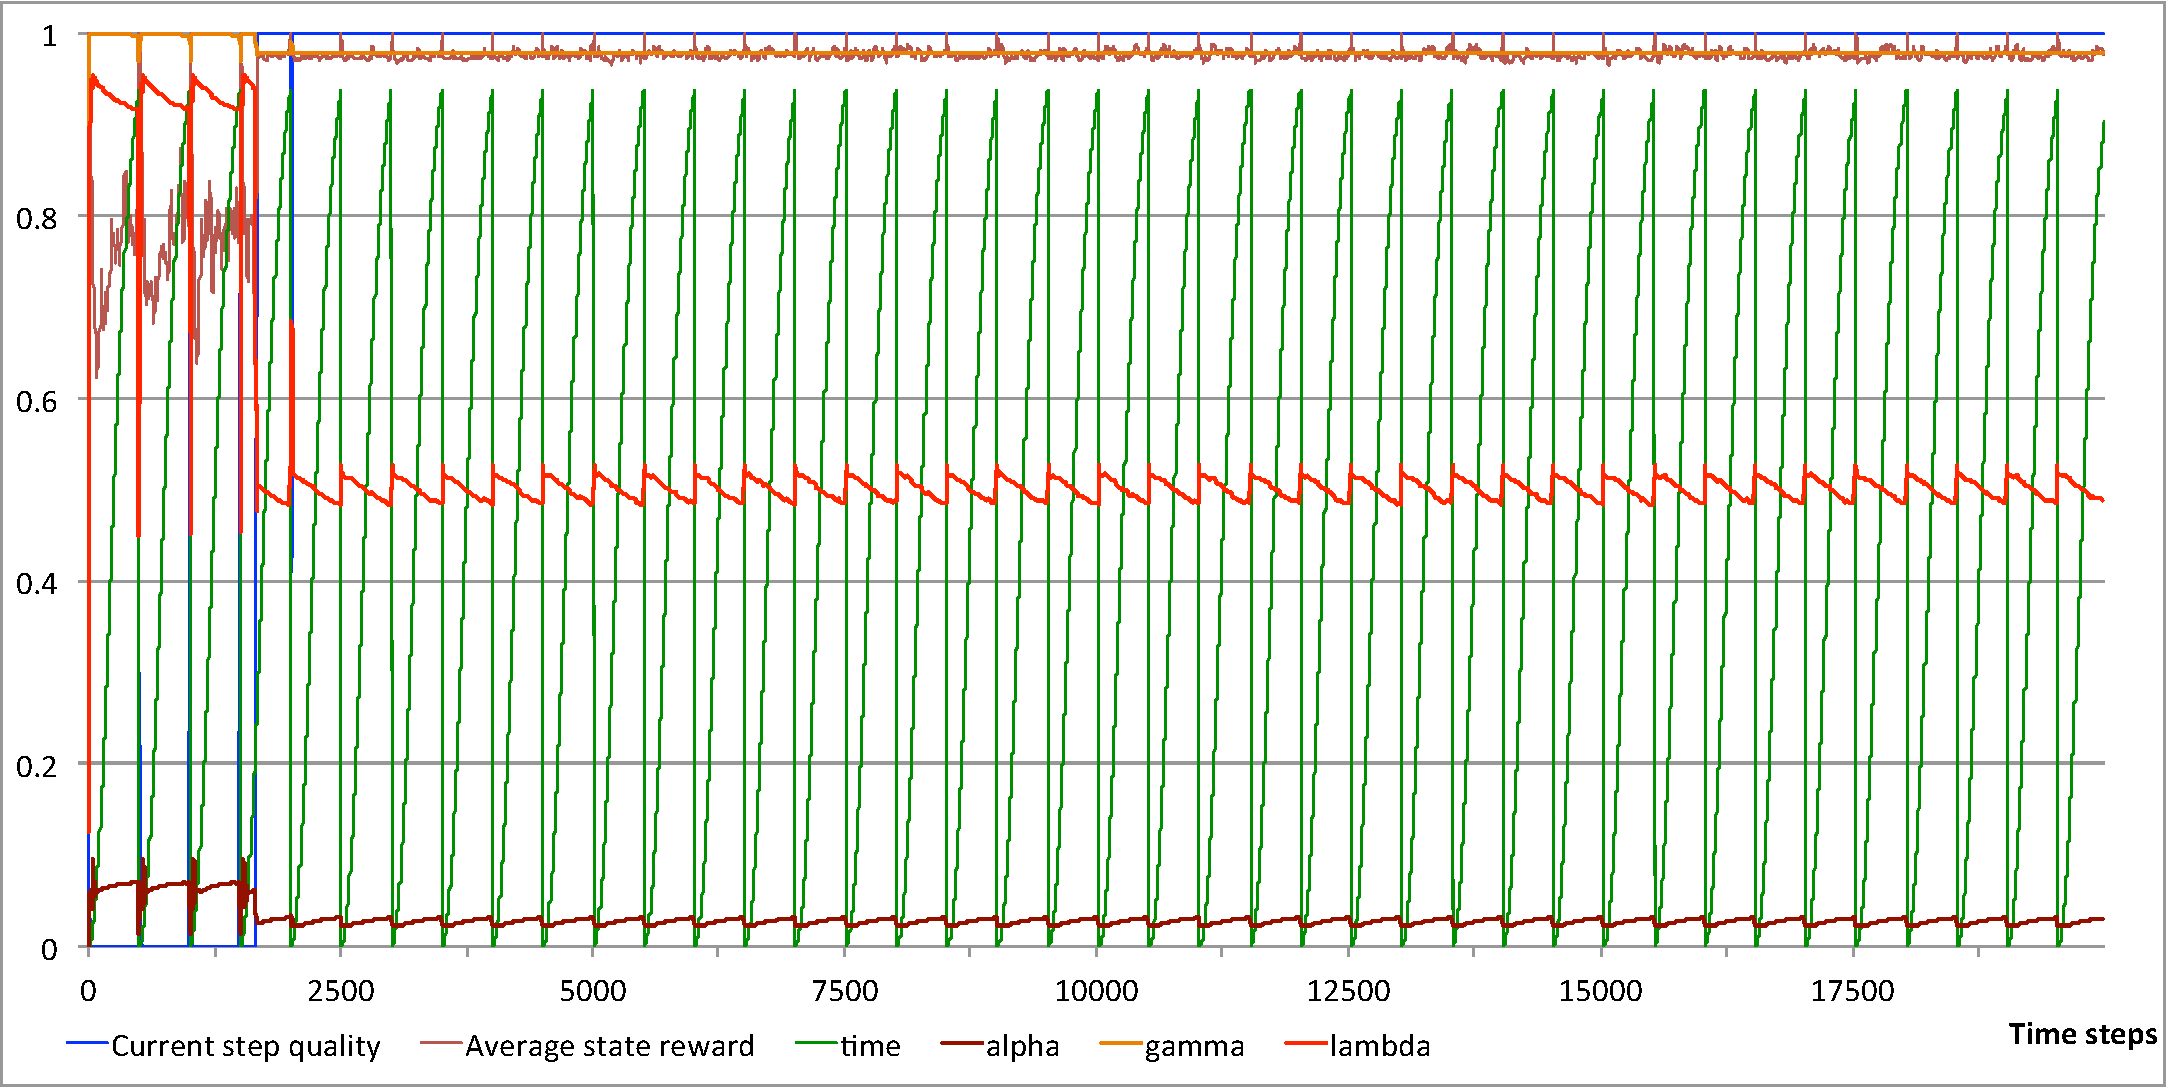
\includegraphics[width=0.245\linewidth]{PW_GRNGenericBehavior.pdf} &
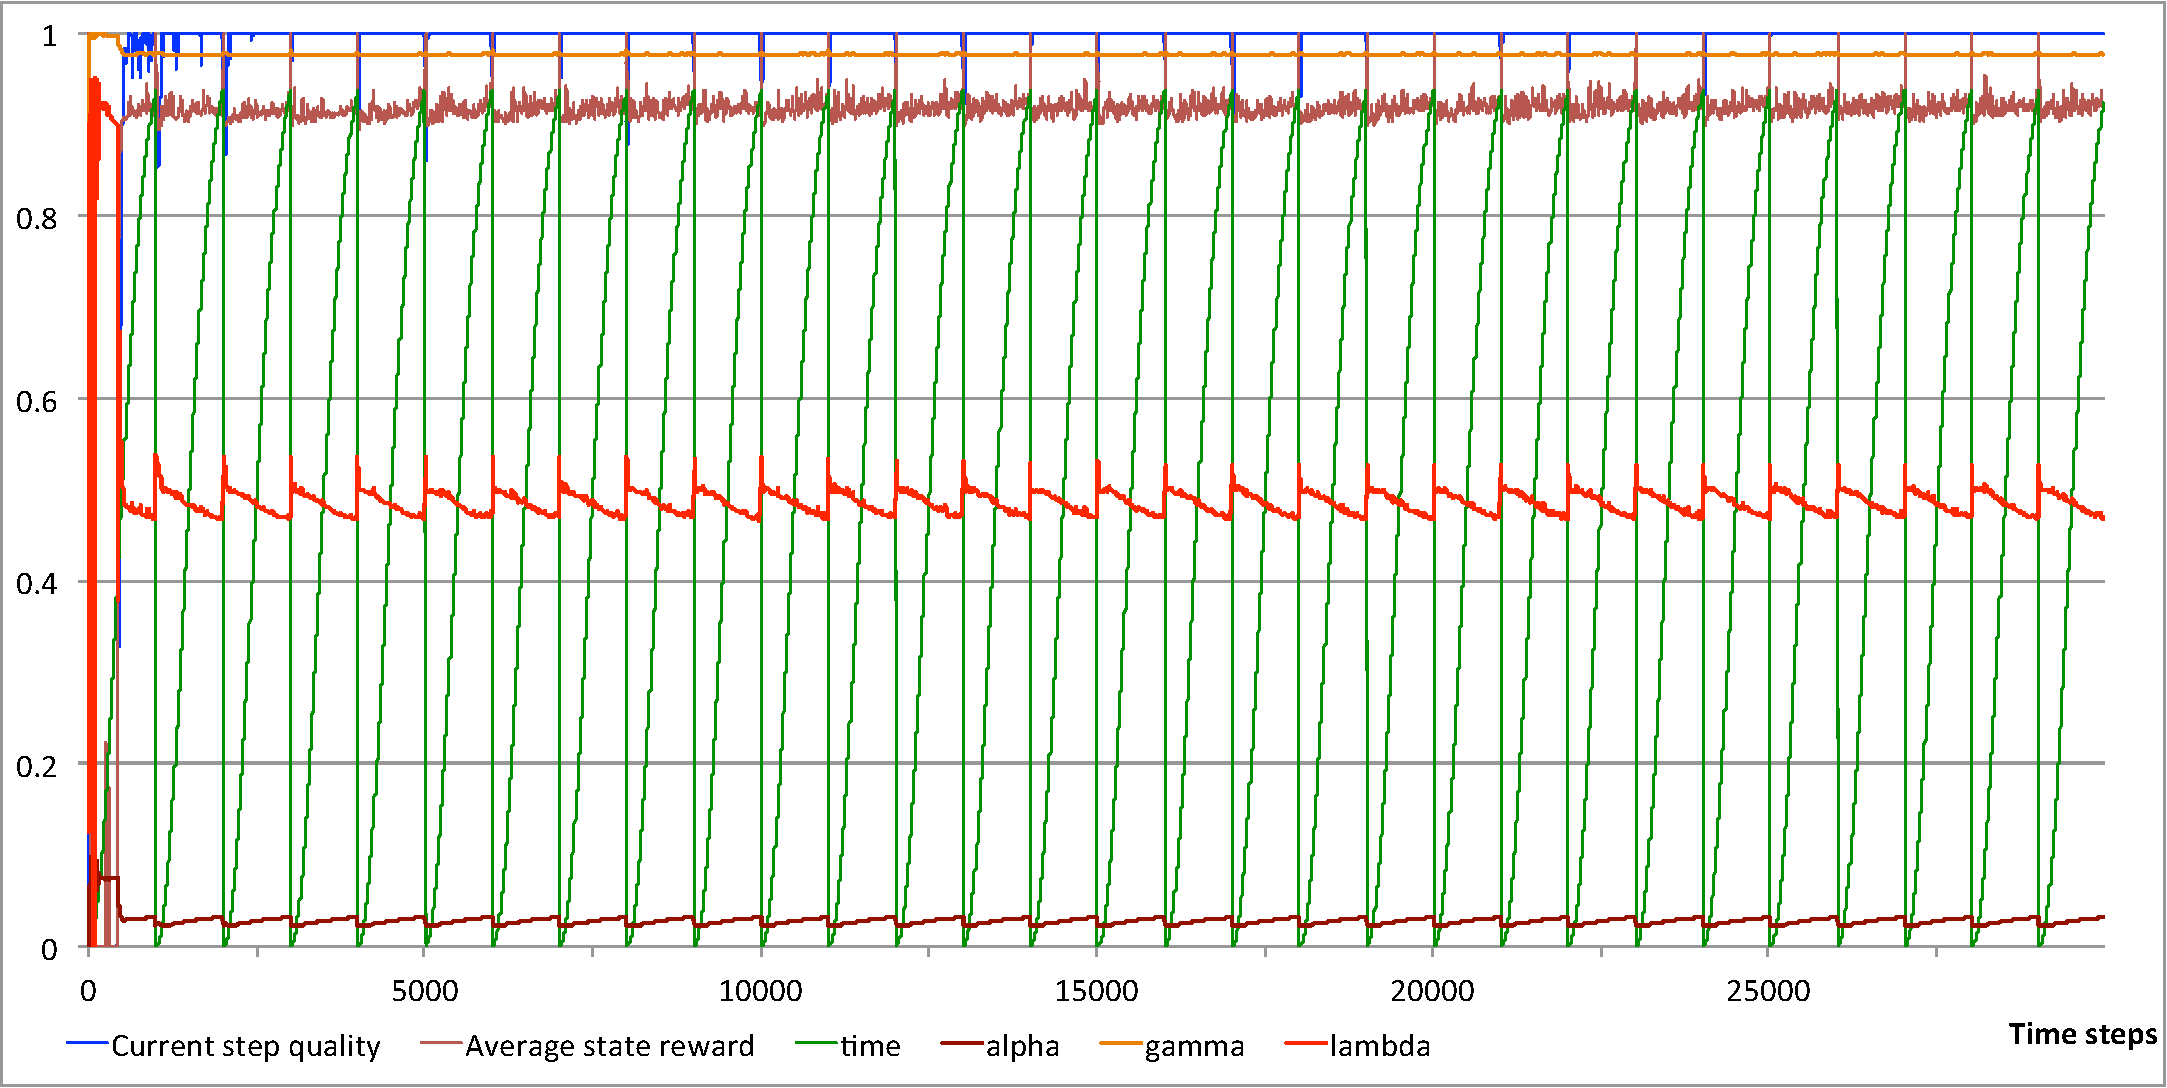
\includegraphics[width=0.245\linewidth]{ACP_GRNGenericBehavior.pdf} \\
(a) Mountain Car & (b) Maze & (c) Puddle World & (d) Acrobat
\end{tabular}
\caption{Behavior of the GRN trained on the Maze and Mountain Car problems when used to regulate learning parameters on other problems.}\label{fig:GRNGenericBehavior}
\end{figure*}

\subsection{Using the GRN trained on Maze}
A powerful property of artificial gene regulatory networks is their capacity to generalize to unknown situations \cite{sanchez2014gene}. In the case of genetically-regulated neuromodulation, we considered the best GRN trained on the maze problem and tested it on other problems. We noticed that it performs well in comparison to the fixed-parameter SARSA algorithm: as presented in Table \ref{tab:results}, GRNM trained on maze (noted GRN$_{m}$) obtains better results than the fixed-parameter SARSA algorithm on all other problems we have tested. In our opinion, the regulatory dynamics of this GRN are very generic: when the rewards start to increase, the learning rate is lowered to preserve previously learned experiences. This regulatory dynamic appears to be appropriate for most problems. However, this generic regulatory network does not beat GRNs trained on specific problems. This can be explained by the fact that optimizing the GRN on an individual problem allows the system to exploit problem-specific features, improving the quality of the parameter regulation.

Figure \ref{fig:all:GRNMazeBehavior} shows the behavior of the GRN trained on the Maze problem and used on other problems. The behaviors are slightly different on each problem: the GRN is able to adapt to problem specificities. In particular, when the episodes are taking to much time, this GRN increases $\lambda$ first and then $\alpha$. It is also interesting to notice that the stabilized values of the learning parameters differ from a problem to another. For example, $\lambda$ is kept around 0.8 on the mountain car problem, around 0.65 for the puddle world and the acrobat problems whereas it is equal to 0.7 on the maze problem. These values have to be compared to the best values obtained for fixed parameters in table \ref{tab:SARSAFixedParams}: it shows the capacity of the GRN to approximate the best learning parameters to a problem without further learning.

When comparing to the fixed-parameter SARSA algorithm and GRNM optimized specifically on one problem (Table \ref{tab:results}), the GRN evolved on Maze outperforms fixed-parameter SARSA on Mountain Car and Acrobat but has poorer results on Puddle World. However, the worst-case is better than fixed-parameter SARSA on all problems, even Puddle World where the average reward is lower. Once again, this shows the capacity of GRNM to compensate learning parameters in harder scenarios.

\subsection{Evolving a generic GRN}
Based on this observation, we have trained a new GRN on two problems instead of only one. The aim is to obtain a generic GRN that has been optimized for multiple problems. We have chosen to train the GRN on the Maze and the Mountain Car problems. Figure \ref{fig:GRNGenericBehavior} shows the behavior of the best GRN obtained. Comparable regulatory behavior can be observed on the different problems: at the beginning of each episode, $\lambda$ is set up to a high value and then reduces until the end of the episode. However, the parameter values are regulated to different levels for each problem. The GRN might use the current step quality and the average state reward inputs to regulate these levels. These inputs provide the GRN with an estimation of the agent's progression in an episode. As the agent progresses further into an episode, the number of sequences of actions that could have led to any given state are almost always increasing, thus when the agent is learning values of states and actions later in an episode it appears to be useful to discount older actions and favor shorter and more recent sequences of actions.

To compare the generic GRN to specific GRNs and to GRNs trained on Maze, we have compared this GRN using the same procedure as with prior experiments: the generic GRN is evaluated on 100 independent runs with different random seeds. Corresponding results are shown in Table \ref{tab:results} as the GRN$_g$ column. Interestingly, the generic GRN beats GRN$_m$ on the Puddle World and Acrobat problems but does not beat the GRNs specifically trained on these problems. The generic GRN and the GRN trained on Maze perform comparably on the Mountain Car problem, but the GRN trained on Maze is doing better on the Maze itself. This was expected since the GRN trained on Maze is specifically optimized for this problem whereas the generic GRN has been trained on two problems and thus its optimization was also affected by training on Mountain Car. Just as the GRN trained on Maze, the generic GRN beats the fixed-parameter SARSA algorithm on the Mountain Car and Acrobat problems. Both the Maze and Puddle World problems favor fixed-parameter SARSA. However, all GRNs do better in the worst-case scenarios due to the ability of GRNs to react to situations dynamically and avoid incorrect credit assignment in sequences of actions (for example, by varying $\lambda$).

